\documentclass[11pt]{article}

% \usepackage{default}
% \usepackage{fullpage}
\usepackage[margin=1in]{geometry}
\usepackage{amsmath}
\usepackage{amssymb}
\usepackage{amsthm}
\usepackage{setspace}
\usepackage{graphicx}
\usepackage{subcaption}
\usepackage{url}
\usepackage{algorithm}
\usepackage{algpseudocode}


\bibliographystyle{plain}

\author{David~Love and G\"{u}zin~Bayraksan}

\title{Two-Stage $\phi$-Divergence Robust Linear Program: Properties and Application to Water Allocation under Uncertainty}
\date{}

% Frequently used general mathematics
\newcommand{\R}{{\mathbb{R}}}
\newcommand{\Rp}{\R^+}
\newcommand{\Z}{{\mathbb{Z}}}
\newcommand{\Zp}{\Z^+}
\newcommand{\Q}{\mathbb{Q}}
\newcommand{\N}{\mathbb{N}}

% Commands for probability
\renewcommand{\P}{\mathbb{P}}
\newcommand{\E}{\mathbb{E}}
\newcommand{\p}[1]{\P \left[ #1 \right]}
\newcommand{\e}[1]{\E \left[ #1 \right]}
\newcommand{\ee}[2]{\E_{#1} \left[ #2 \right]}

% Definitions of variables
\newcommand{\X}{X}
\newcommand{\x}{\mathbf{x}}
\newcommand{\xh}{\hat{\x}}
\newcommand{\lh}{\hat{\lambda}}
\newcommand{\mh}{\hat{\mu}}
\newcommand{\xs}{\x^*}
\newcommand{\xit}{\tilde{\mathbf{\xi}}}
\newcommand{\zt}{\tilde{z}}
\newcommand{\zs}{z^*}

% Further variables
\newcommand{\y}{\mathbf{y}}
\renewcommand{\c}{\mathbf{c}}
\newcommand{\q}{\mathbf{q}}
\renewcommand{\b}{\mathbf{b}}
\renewcommand{\d}{\mathbf{d}}

% Epiconvergence for \plp
\newcommand{\ptrue}{p^{\text{true}}}

% Useful mathematics functions
\newcommand{\keywords}[1]{\par\noindent\enspace\ignorespaces\textbf{Keywords:} #1}
% \newcommand{\keywords}[1]{\par\addvspace\baselineskip\noindent\keywordname\enspace\ignorespaces #1}
\DeclareMathOperator*{\argmin}{argmin}
\newtheorem{theorem}{Theorem}
\newtheorem{lemma}[theorem]{Lemma}
\newtheorem{proposition}[theorem]{Proposition}
\newtheorem{corollary}[theorem]{Corollary}
\newtheorem{remark}[theorem]{Remark}
\newtheorem{definition}[theorem]{Definition}
\newcommand{\st}{\mbox{s.t.}}

% Naming shortcuts
\newcommand{\plp}{$\phi$LP-2}

\begin{document}

\maketitle

\begin{abstract}
	We adapt and extend the likelihood robust optimization method recently proposed by Wang, Glynn, and Ye to a two-stage setting.
	We examine the value of collecting additional data and the cost of finding a solution robust to an ambiguous probability distribution.
	A decomposition-based solution algorithm to solve the resulting model is given.
	We apply the model to examine a long-term water allocation problem in the southeast area of Tucson, AZ under ambiguous distribution of future available supply and demand and present computational results.
\end{abstract}

\keywords{Optimization under uncertainty, water resources management,  ambiguous stochastic programming, robust optimization, environmental sustainability}

\section{Introduction and Motivation}

% More than 25 million people in the southwestern United States depend on the water supplied by the Lower Colorado River Basin for their livelihood.
% More than half of Tucson's water, for instance, comes from this source.
% The Colorado River Basin has experienced a sustained period of drought in recent years, which has led to questions about the adequacy of the Colorado to meet future demands, especially as the population of Arizona (and of other states that depend on this water source) increases.
% Thus, the problem of allocating Colorado water is of critical importance. 
 
% The reliability of the Colorado River system under future climate variability is critically important to the long-term well-being of Arizona and the other six states that depend on this water supply \cite{usbr_colorado_climate}. 
% The current approach to modeling the water supply is to use Global Circulation Models (GCM) to generate regional rainfall and temperature scenarios by the so-called statistical downscaling techniques \cite{christensen_lettenmaier_07,dibike_caulibaly_05}.  
% The US Bureau of Reclamation also uses an approach called the {\it scenario planning} that examines water demand and supplies over the next 50 years \cite{usbr_11}.

In practice, many optimization problems can be modeled by stochastic programs minimizing an expected value of an uncertain objective function.
However, if the distribution of the uncertain parameters used in the model is incorrect, the stochastic program can give highly suboptimal results.
Such problems have led to the development of distributionally robust optimization, a modeling technique that replaces the probability distribution by a set of distributions, and optimizes the expected cost relative to the worst distribution in the uncertainty set.
One approach to this has been recently proposed by Wang, Glen and Ye \cite{wang2010likelihood} is to use a set of distributions that are within a sufficiently high empirical likelihood for a given set of observations.
The result is called the Likelihood Robust Optimization (LRO) method.
In this paper, we adapt and extend LRO to a more general two-stage stochastic linear program with recourse, and examine the properties of the resulting model.
We then develop a simple condition for assessing the value of collecting extra data.
Finally, we develop a modified Bender's Decomposition to solve the LRO and apply the above results to a water distribution planning problem.

Stochastic programs with uncertain objective functions have long been studied by applying the minimax approach to an expected cost \cite{dupacova_87}.
Shapiro and Kleywegt \cite{shapiro2002minimax} and Shapiro and Ahmed \cite{shapiro2004class} developed methods for converting stochastic minimax problems into equivalent stochastic programs with a certain distribution.

Distributionally robust methods have been drawing considerable attention in recent years.
Erdo{\u{g}}an and Iyengar \cite{erdogan2006ambiguous} studied chance-constrained stochastic programs where the set of distributions considered is determined by the Prohorov metric.
Calafiore and Campi \cite{calafiore2005uncertain} developed a data-driven method for generating feasible solutions to chance constrained problems, and later Calafiore and El Ghaoui \cite{calafiore2006distributionally} developed a method for converting distributionally robust chance constraints into second-order cone constraints.
Jiang and Guan \cite{jiang2012data} developed an exact approach to solving data-driven chance constrained programs.
Delage and Ye \cite{delage_ye_10} provide methods for modeling uncertain distributions of a specific form (e.g., Gaussian, exponential, etc.) or using moment-based constraints.
Ben-Tal \cite{bental2011robust} studies distributionally robust stochastic programs when the uncertainty region is defined by selecting distributions using a $\phi$-divergence.
The method of Likelihood Robust Optimization proposed in \cite{wang2010likelihood} that we adapt in this paper is a special case of the $\phi$-divergence measures of \cite{bental2011robust}.

The LRO is an attractive approach because the uncertainty set of distributions is determined by the Kullback-Leibler divergence from a ``nominal'' distribution.
Furthermore, only those scenarios of interest are used directly in the calculations.
These scenarios can come from direct observation, results of simulation, from expert opinion regarding scenarios that the decision maker would especially like to be robust against.
Because the LRO depends only on these scenarios, the size of the problem is polynomial in the sample size, making it computationally tractable.

We apply LRO to a generalized network model of Colorado River water allocation in Tucson, Arizona motivated by the CALVIN (CALifornia Value Integrated Network) optimal water allocation model of California created by Draper et al.\ \cite{draper_etal_03}.
Other models of Colorado River water distribution have also been studied, such as the Colorado River Reservoir Model \cite{christensen2004effects} and the Colorado River Budget Model \cite{barnett2009sustainable}.

This paper is organized as follows: Section \ref{sec:lrlp2} presents the extension of LRO model to a two-stage stochastic program with recourse.
Section \ref{sec:properties} describes basic properties of LRO;
Section \ref{sec:robust_level} gives a method of selecting the level of robustness;
Section \ref{sec:value} discusses the value of collecting additional data;
and Section \ref{sec:epiconvergence} discusses the asymptotic properties of LRO.
In Section \ref{sec:soln_algorithm} we present a decomposition method for solving the LRO model; and in Section \ref{sec:comp_results} we present a generalized network water model and computational results for its LRO model.
Finally, we end in Section \ref{sec:concl} with conclusions and future work.


%%%%%%%%%%%%%%%%%%%%%%%%%%%%%%%%%%%%%%%%%%%%%%%%%%%%%%%%%%%%%%%%%%%%%%%%%%%%%%%%
\section{\plp\ Formulation}
\label{sec:lrlp2}

We begin with a two-stage stochastic linear program with recourse (SLP-2).
Let $\x$ be a vector of of first stage decision variables with cost vector $\c$, constraint matrix $A$ and right hand side $\b$.
We assume a finite distribution given by $p_\omega$ with scenarios indexed by $\omega = 1, \dots, n$.
The SLP-2 is
\begin{align}
	\min_\x \ & \left\{ \c\x + \sum_{\omega=1}^n p_\omega h_\omega(\x) : A\x = b, \x \geq 0 \right\} \label{eq:slp_first_stage}% \\
% 	\st \ & A\x = \b \nonumber  \\
% 	&\ \ \ \x \geq 0 \nonumber
\end{align}
where
\begin{align}
	h_\omega(\x) = \min_{y^\omega} \ & \left\{ \q^\omega y^\omega : D^\omega y^\omega = B^\omega \x + \d^\omega, y^\omega \geq 0 \right\} \label{eq:slp_second_stage}% \\
% 	\st \ & D^\omega y^\omega = B^\omega \x + \d^\omega \nonumber \\
% 	& \ \ \ y^\omega \geq 0. \nonumber
\end{align}
We assume relatively complete recourse; i.e., the second-stage problems $h_\omega(\x)$ are feasible for every feasible solution $\x$ of the first-stage problem; and that the second-stage problems $h_\omega(\x)$ are dual feasible for every feasible solution $\x$ of the first-stage problem..

The SLP-2 formulation assumes that the distribution $\{p_\omega\}_{\omega=1}^n$ is known.
However, in many applications, including our water planning, the distribution is itself unknown.
One technique to deal with this is to replace the known distribution with an {\it ambiguity set} of distributions; i.e., a set of distributions which is believed to contain the true distribution.
Ben-Tal et.\ al.\ \cite{bental2011robust} proposed at the ambiguity set could be generated with $\phi$-divergences, including only those distributions whose divergence from the nominal distribution $\{q_\omega\}_{\omega=1}^n$ is sufficiently small.
Throughout much of this paper, we assume that $\{q_\omega\}$ is generated from observations, where scenario $\omega$ has been observed $N_\omega$ times, with $N = \sum_{\omega=1}^n N_\omega$ total observations, leading to the empirical distribution $\hat{p}^N_\omega = N_\omega / N$.
In SLP-2, this would correspond to probability of scenario $\omega$ to be $\hat{p}_\omega$.
By replacing the specific distribution in SLP-2 with a set of distributions with sufficiently close to the nominal distribution in the $\phi$-divergence sense, we create a model that we refer to as two-stage $\phi$-divergence linear program with recourse (\plp).

To derive the \plp, we begin by writing SLP-2 given in \eqref{eq:slp_first_stage}--\eqref{eq:slp_second_stage} in extensive form
\[
	\begin{array}{rrrl}
		\min_{\x,y^\omega} \ & \c\x & + \sum_\omega p_\omega \q^\omega y^\omega \label{eq:slp2cost} \\
		\st \ & A\x & & = \b \nonumber \\
		& -B^\omega \x & + D^\omega y^\omega & = \d^\omega,\ \forall \omega \nonumber \\
		& \x & & \geq 0 \nonumber \\
		& & y^\omega & \geq 0,\ \forall \omega. \nonumber
	\end{array}
\]
The SLP-2 formulation is then augmented by the set of distributions with sufficiently low divergence from $\{q_\omega\}$.
To be robust against all these possible distributions, the distribution that results in the maximum expected cost is considered.
Then, the objective function is minimized with respect to this worst-case distribution selected from the ambiguity set of distributions.
The resulting minimax formulation of \plp\ is
\begin{align}
	\min_{\x,y^\omega} \max_p \ & \c\x + \sum_\omega p_\omega \q^\omega y^\omega \label{eq:plp_primal}\\
	\st \ & A\x = \b, \x \geq 0 \nonumber \\
	& -B^\omega \x + D^\omega y^\omega = \d^\omega,\ \forall \omega \nonumber \\
	& \sum_\omega q_\omega \phi\left(\frac{p_\omega}{q_\omega}\right) \leq \rho \label{eq:plp_primal_divergence} \\
	& \sum_\omega p_\omega = 1 \label{eq:plp_primal_probability} \\
	& \x \geq 0 \nonumber \\
	& y^\omega, p_\omega \geq 0,\ \forall \omega. \label{eq:nonneg}
\end{align}

Taking the dual of the inner maximization problem, with dual variables $\lambda$ and $\mu$, of constraints (\ref{eq:plp_primal_divergence}) and (\ref{eq:plp_primal_probability}), respectively, yields
\begin{align*}
	\min_{\lambda,\mu} \ & \mu + \rho \lambda + \lambda \sum_\omega q_\omega \phi^*\left(\frac{\q^\omega y^\omega - \mu}{\lambda}\right) \\
	\st \ & \lambda \geq 0 \\
	& \frac{\q^\omega y^\omega - \mu}{\lambda} \leq \lim_{t \rightarrow \infty} \frac{\phi(t)}{t}, \ \forall \omega,
\end{align*}
See Theorem 1 of \cite{bental2011robust} for a derivation of the derivation of the dual problem.
Note in particular that the dual formulation is accurate even for $q_\omega = 0$ for some $\omega$.

Combining the two minimizations gives \plp\ in extensive form
\begin{align}
	\min_{\x,\lambda,\mu,y^\omega} \ & \c\x + \mu + \rho \lambda + \sum_\omega q_\omega \phi^*\left(\frac{\q^\omega y^\omega - \mu}{\lambda}\right) \nonumber \\
	\st \ & A\x = \b \nonumber \\
	& -B^\omega \x + D^\omega y^\omega = \d^\omega,\ \forall \omega \label{eq:plp_det_equiv} \\
	& \frac{\q^\omega y^\omega - \mu}{\lambda} \leq \lim_{t \rightarrow \infty} \frac{\phi(t)}{t}, \ \forall \omega \nonumber \\
	& \x,\lambda,y^\omega \geq 0, \ \forall \omega. \nonumber
\end{align}

Finally, we wish to return the \plp\ to two-stage formulation.
\begin{align}
	\min_{\x,\lambda,\mu} \ & \c\x + \mu + \rho \lambda + \sum_\omega q_\omega \phi^*\left(\frac{h_\omega(\x) - \mu}{\lambda}\right) \nonumber \\
	\st \ & A\x = \b \label{eq:plp_two_stage} \\
	& \frac{\q^\omega y^\omega - \mu}{\lambda} \leq \lim_{t \rightarrow \infty} \frac{\phi(t)}{t}, \ \forall \omega \label{eq:plp_feas_constraint}\\
	& \x,\lambda \geq 0, \nonumber
\end{align}
where
\begin{align}
	h_\omega(\x,\lambda,\mu) = \q^\omega y^\omega \label{eq:plp_second_stage} \\
	\st \ & -B^\omega \x + D^\omega y^\omega = \d^\omega \nonumber \\
	& y^\omega \geq 0. \nonumber
\end{align}

%%%%%%%%%%%%%%%%%%%%%%%%%%%%%%%%%%%%%%%%%%%%%%%%%%%%%%%%%%%%%%%%%%%%%%%%%%%%%%%%
\section{Basic Properties of \plp}
\label{sec:properties}

In this section, we list some basic properties of \plp.
Most of these have already been noted in \cite{bental2011robust}, with a special case noted in \cite{wang2010likelihood}, but we list them for completeness and some of these properties help with our special solution method.

\subsection{Coherent Risk Measure}
As noted in \cite{wang2010likelihood}, the \plp\ problem can be viewed as minimizing a coherent risk measure.
A coherent risk measure (in the basic sense), as defined in \cite{rockafellar2007coherent}, is a functional ${\cal R}: L^2 \rightarrow (-\infty,\infty]$ defined on random variables such that
\begin{enumerate}
	\item ${\cal R}(C) = C$ for all constants $C$,
	\item ${\cal R}((1-\lambda)X + \lambda X') \leq (1-\lambda){\cal R}(X) + \lambda {\cal R}(X')$, i.e., $\cal R$ is convex,
	\item ${\cal R}(X) \leq {\cal R}(X')$ when $X \leq X'$, i.e., $\cal R$ is monotonic,
	\item ${\cal R}(\lambda X) = \lambda {\cal R}(X)$ for $\lambda > 0$, i.e., $\cal R$ is positively homogeneous.
\end{enumerate}

\begin{proposition}
	\plp\ is equivalent to minimizing a coherent risk measure.
\end{proposition}

\begin{proof}
	Rockafellar also shows that $\cal R$ is a coherent risk measure if and only if it can be written using a risk envelope \cite{rockafellar2007coherent}.
	We will show that \plp\ can be written in the form of a risk envelope in the primal form (\ref{eq:plp_primal}) with the change of variables $\tilde{p}_\omega = \frac{p_\omega}{1/n}$.
	Throughout the proof, all expectations are taken with respect to the uniform distribution.
	
	First, probability constraint (\ref{eq:plp_primal_probability}) can be written as $\e{\tilde{p}} = 1$, where $\tilde{p}$ is the random variable taking values $\tilde{p}_\omega$ with equal probability.
	Then the $\phi$-divergence constraint (\ref{eq:plp_primal_divergence}) becomes $\sum_{\omega=1}^n \frac{1}{n} \tilde{p}_\omega \frac{\phi\left(\tilde{p}_\omega/\tilde{q}_\omega\right)}{\tilde{p}_\omega/\tilde{q}_\omega} \leq \rho$, where $\tilde{q}_\omega = \frac{q_\omega}{1/n}$ and $\frac{\phi(a/0)}{a/0} = \lim_{t \rightarrow \infty} \frac{\phi(t)}{t}$.
	Combining these yields the set ${\cal Q} = \{\tilde{p} | \e{\tilde{p}} = 1, sum_{\omega=1}^n \frac{1}{n} \tilde{p}_\omega \frac{\phi\left(\tilde{p}_\omega/\tilde{q}_\omega\right)}{\tilde{p}_\omega/\tilde{q}_\omega} \leq \rho \}$, a closed and convex risk envelope.
	Finally, we can rewrite the inner maximization of (\ref{eq:plp_primal}) as $\max_{\tilde{p} \in {\cal Q}} \e{\tilde{p} h(x)}$, where $h(x)$ is the random variables defined by $\{h_\omega(x)\}$.
	Thus we see that \plp\ is the minimum of a coherent risk measure.
\end{proof}

\begin{remark}
	The above proof can be simplified by using $\tilde{p}_\omega = \frac{p_\omega}{q_\omega}$ if $q_\omega > 0$ for all $\omega$.
	However, the case of $q_\omega = 0$ plays an important roll in the classification presented in Section \ref{sec:classification}.
\end{remark}


Note that being a coherent risk measure implies that \plp\ is a convex problem.
The convexity of LRO was also noted in \cite{wang2010likelihood}.

\subsection{Time Structure}
The second-stage problems are unaffected by the change from SLP-2 to \plp.
This preservation of the time structure allows us to easily convert \mbox{(sub-)derivatives} of $h_\omega(\x)$ to \mbox{(sub-)derivatives} of $\phi^*\left(\frac{h_\omega(\x) - \mu}{\lambda}\right)$.
We will use this in the decomposition method provided in Section \ref{sec:soln_algorithm}.

\subsection{Primal-Dual Variable Relationships}
The appearance of the conjugate $\phi^*(s)$ in the objective of (\ref{eq:plp_two_stage}) gives the method retrieving the worst-case distribution,
\begin{equation} \label{eq:p_worst}
	\frac{p_\omega}{q_\omega} \in \partial \phi^*\left(\frac{h_\omega(\x)-\mu}{\lambda}\right).
\end{equation}
If $q_\omega = 0$, then either $p_\omega = 0$ or $\infty \in \partial \phi^*\left(\frac{h_\omega(\x)-\mu}{\lambda}\right)$.

%%%%%%%%%%%%%%%%%%%%%%%%%%%%%%%%%%%%%%%%%%%%%%%%%%%%%%%%%%%%%%%%%%%%%%%%%%%%%%%%
\section{The Level of Robustness}
\label{sec:robust_level}

The literature on $\phi$-divergences provides some insight on choosing a reasonable asymptotic value of $\rho$.
Theorem 3.1 of \cite{pardo2005statistical} shows that the statistic $T^\phi_N(\hat{p},\ptrue) = \frac{2N}{\phi''(1)} \sum_{\omega=1}^n \ptrue_\omega \phi\left(\frac{\hat{p}_\omega}{\ptrue_\omega}\right)$ converges in distribution to a $\chi^2$-distribution with $n-1$ degrees of freedom.
Ben-Tal \cite{bental2011robust} then uses this result to suggest the asymptotic value
\begin{equation} \label{eq:asymptotic_rho}
	\rho = \frac{\phi''(1)}{2N} \chi^2_{n-1,1-\alpha},
\end{equation}
where $\chi^2_{n-1,1-\alpha}$ is the $1-\alpha$ percentile of a $\chi^2_{n-1}$ distribution, which produces an approximate $1-\alpha$ confidence region on the true distribution.

% Wang et. al. \cite{wang2010likelihood} suggest a Bayesian interpretation of the likelihood constraint (\ref{eq:plp_primal_divergence}) which yields a Monte Carlo method for establishing a value for $\gamma'$.
% Considering the observations $\{N_\omega\}$ and empirical probabilities $\hat{p}^N_\omega = \frac{N_\omega}{N}$ as fixed, Wang et. al. \cite{wang2010likelihood} introduce a distribution $\P^*$ on the $n$-dimensional simplex whose density is proportional to the likelihood $\prod_\omega p_\omega^{N_\omega}$.
% This is the Dirichlet distribution $Dir(\beta)$, which has density
% \[
% 	\frac{1}{B(\beta)} \prod_{\omega=1}^n p_\omega^{\beta_\omega-1}
% \]
% where the normalizing factor is $B(\beta) = \frac{\prod_{\omega=1}^n \Gamma(\beta_\omega)}{\Gamma\left( \sum_{\omega=1}^n \beta_\omega \right)}$.
% The unknown true distribution can then be modeled as coming from a $Dir(\beta)$ distribution with parameters $\beta_\omega = N_\omega + 1$.
% The parameter $\gamma'$ is chosen such that $\P^*\left\{ \prod_{\omega=1}^n p_\omega^{N_\omega} \geq \gamma' \prod_{\omega=1}^n (\hat{p}^N_\omega)^{N_\omega} \right\}$.
% This probability can be estimated by Monte Carlo sampling.
% 
% Figure \ref{fig:gammaprime_by_sample} shows the estimated values of $\gamma'$ for a $95\%$ confidence region for distributions with $n = 10$ scenarios.
% You can notice four distinct, color-coded ``bands'' of values of $\gamma'$.
% These bands are determine by the size of the set $\{\omega | N_\omega = 0\}$, i.e., the number of scenarios which have not been sampled.
% The highest band, in blue, has all $N_\omega > 0$.
% The next (green) band has one $N_\omega = 0$, followed by red with two and cyan with three.
% 
% \begin{figure}
% 	\centering
% 	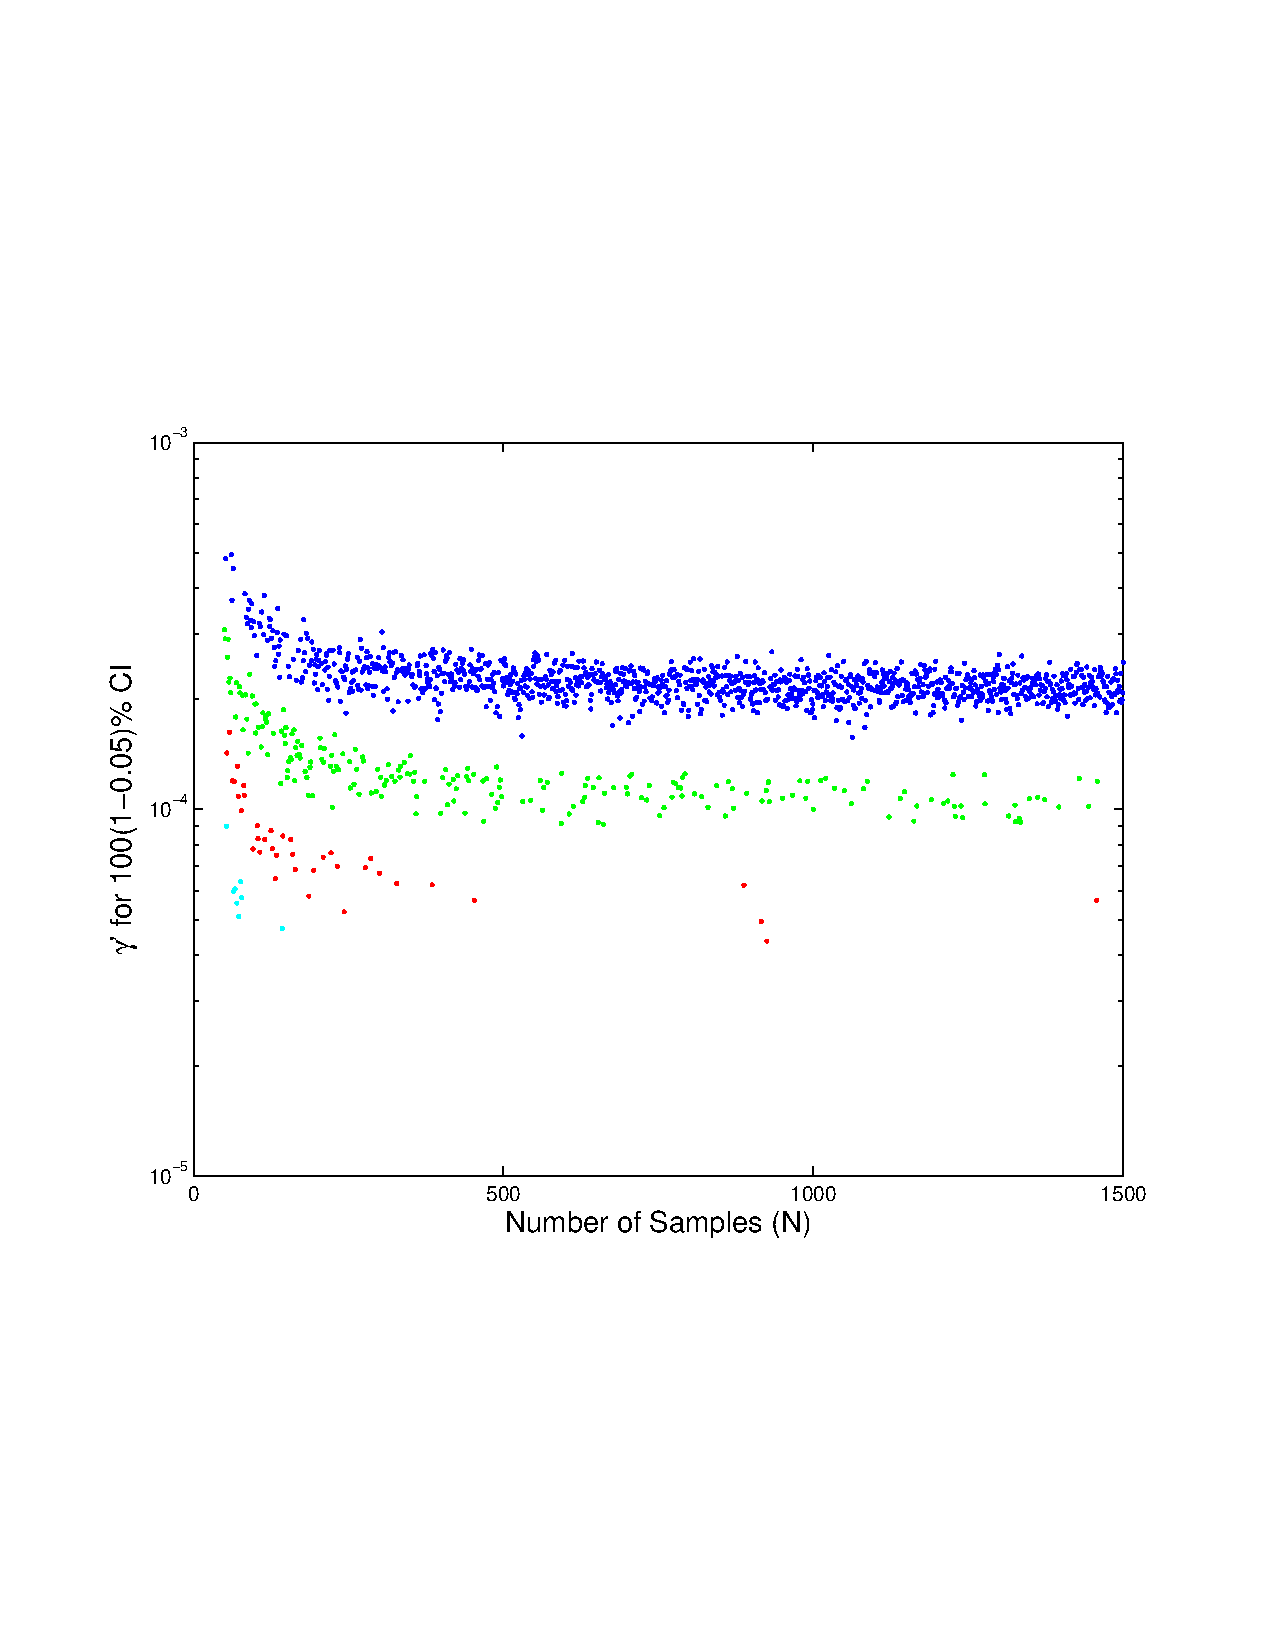
\includegraphics[width=.6\textwidth]{images/gammaprime_diff_samples_dim_10}
% 	\caption{
% 		Computed estimates for $\gamma'$ to achieve a $95\%$ confidence region using the Dirichlet distribution.
% 		Each point estimate was computed using a randomly generated $n=10$ dimensional probability distribution from which $N$ samples were selected.
% 		The value of $\gamma'$ was estimated by Monte Carlo sampling from $Dir(\beta)$ with $\beta_\omega = N_\omega + 1$.
% 		The color indicates how many of the $n$ scenarios were not represented in the $N$ samples: blue indicates that all $N_\omega > 0$, green has exactly one $N_\omega = 0$, red has two, and cyan has three.
% 	}
% 	\label{fig:gammaprime_by_sample}
% \end{figure}

%%%%%%%%%%%%%%%%%%%%%%%%%%%%%%%%%%%%%%%%%%%%%%%%%%%%%%%%%%%%%%%%%%%%%%%%%%%%%%%%
\section{Classification of $\phi$-Divergences}
\label{sec:classification}

We present a classification of $\phi$-divergences into four types, resulting from an examination of the limiting behavior of $\phi(t)$ as $t \rightarrow 0$ and $t \rightarrow \infty$.
Different classifications may be suitable to different problem types and desired qualities in the ambiguous model.

As motivation, consider a self-adjoint $\phi$-divergence, which satisfies the relation
\begin{equation} \label{eq:self_adjoint_classification}
	\frac{\phi(t)}{t} = \phi\left(\frac{1}{t}\right),
\end{equation}
and consider $t \rightarrow \infty$.
If both sides of (\ref{eq:self_adjoint_classification}) are finite in the limit, then we see a similarity between the boundedness of $\phi(t)$ for $t < 1$ and linear growth of $\phi(t)$ for $t > 1$.
On the other hand, infinite limits of (\ref{eq:self_adjoint_classification}) indicate a similarity between superlinear growth of $\phi(t)$ for $t > 1$ and no bound on $\phi(t)$ for $t < 1$.

In the \plp, $\phi$ has arguments given by ratios of probabilities, $\tfrac{p_\omega}{q_\omega}$, and the limits $t \rightarrow 0$ and $t \rightarrow \infty$ correspond to the cases when $p_\omega = 0$ and $q_\omega = 0$, respectively.
Consider each of these limiting cases:
\begin{itemize}
	\item $p_\omega = 0$ but $q_\omega > 0$ ($\lim_{t \searrow 0} \phi(t)$):
	\begin{itemize}
		\item If $\lim_{t \searrow 0} \phi(t) = \infty$, the ambiguity region will never contain distributions with $p_\omega = 0$ but $q_\omega > 0$.
		\item On the other hand, if $\lim_{t \searrow 0} \phi(t) < \infty$, the ambiguity region could contain such a distribution, provided $q_\omega$ is sufficiently small.
			We say that such a distribution can \emph{suppress} scenario $\omega$.
	\end{itemize}
	\item $p_\omega > 0$ but $q_\omega = 0$ ($\lim_{t \nearrow 0} \frac{\phi(t)}{t}$):
	\begin{itemize}
		\item If $\lim_{t \nearrow 0} \frac{\phi(t)}{t} = \infty$, the ambiguity region will never contain distributions with $p_\omega > 0$ but $q_\omega = 0$.
		\item On the other hand, if $\lim_{t \nearrow 0} \frac{\phi(t)}{t} < \infty$, the ambiguity region will admit sufficiently small $p_\omega$.
			We say that such a distribution can \emph{pop} scenario $\omega$.
	\end{itemize}
	\item $p_\omega = 0$ but $q_\omega = 0$: Such a situation has no contribution to the divergence, since $0 \phi\left(\tfrac{0}{0}\right) = 0$.
\end{itemize}

These two categories describing suppressing and popping behavior in $\phi$-divergences create four distinct categories.
Examples of divergences in each category are given in Table \ref{tb:phi_categories}.

\begin{table}
	\centering
	\begin{tabular}{l|p{.3\textwidth}p{.3\textwidth}}
		 & Can Suppress Scenarios & Cannot Suppress Scenarios \\
		 \hline
		 Can Pop Scenarios %
			& \parbox{.3\textwidth}{Hellinger} %
			& \parbox{.3\textwidth}{Burg Entropy,\\$\chi^2$-distance} \\
		 Cannot Pop Scenarios %
			& \parbox{.3\textwidth}{Kullback-Leibler divergence,\\Modified $\chi^2$-distance} %
			& \parbox{.3\textwidth}{J-Divergence}
	\end{tabular}
	\caption{
		Examples of $\phi$-divergences fitting into each category.
	}
	\label{tb:phi_categories}
\end{table}

\subsection{Modeling Considerations When Choosing a Divergence}

We offer some suggestions for choosing an appropriate $\phi$-divergence classification for the data available.
First, consider whether to choose a distribution that can suppress scenarios.
If the problem scenarios come from high-quality observed data, you may wish to avoid divergences that can suppress scenarios.
However, if the data in poorly sampled, or comes from opinion rather than observation of simulation, it may be desirable to have the option of suppressing scenarios may result in a solution with better robustness properties.

Next, consider whether to choose a distribution that allows for popping scenarios.
If the problem scenarios come strictly from observation, with little theoretical understanding of the problem, we suggest choosing a divergence that cannot pop scenarios.
However, if the problem scenarios come from a mix of observed/simulated data and expert opinion about possibilities of interest, then divergences that can pop scenarios present an interesting modeling choice.
This allows for including interesting but unobserved scenarios, and allowing the mathematical program to assign an appropriate probability to them.

\subsection{Additional Details about Divergences that can Suppress}

Suppressing a scenario is made possible by having $\lim_{t \searrow 0} \phi(t) < \infty$, but there are two further possibilities for such divergences: (1) $\phi'(0) < \infty$ and (2) $\lim_{t \searrow 0} \phi'(t) = \infty$.
This subclassification leads to two different behaviors in $\phi^*(s)$: either (1) $\phi^*(s) = c$ for some constant $c < 0$ and  $s < \underline{s}$; or (2) $\phi^*(s) \searrow c$ as $s \rightarrow -\infty$ asymptotically, but never reaches the bound.
By the primal-dual variable relation $p_\omega = q_\omega \phi^{*\prime}(s_\omega) = q_\omega \phi^{*\prime}\left(\frac{h_\omega(x) - \mu}{\lambda}\right)$, we see two different possibilities for suppressing scenarios:
\begin{enumerate}
	\item If $\phi'(0) < \infty$, then all scenarios that satisfy the relation $h_\omega(x) \leq \mu + \underline{s}\lambda$ are suppressed.
		As $\rho$ increases, scenarios tend to be suppressed one at a time.
	\item Otherwise, scenarios can only be suppressed if $s_\omega = -\infty$, which can only occur if $\lambda = 0$.
		Consequently, this solution must also have $\mu = \max_\omega h_\omega(x)$ in order to maintain a probability distribution.
		This also means that all but the most expensive scenario(s) will vanish simultaneously.
		Divergences of this type can be difficult to deal with numerically when suppression occurs.
\end{enumerate}

\subsection{Additional Details about Divergences that can Pop}

Divergence that can pop a scenario have $\phi(t)$ that grow linearly as $t \rightarrow \infty$, which causes the existence of an upper bound $\bar{s}$ on the domain of $\phi^*(s)$.
The primal-dual variable relation specifies $\frac{p_\omega}{q_\omega} = \partial \phi^*(s_\omega)$, but the left-hand side is undefined when $q_\omega = 0$.
Thus, popping a scenario can only occur when the right-hand side may also be undefined, i.e., when $s_\omega = \bar{s}$, for which $\infty \in \partial \phi^*(s_\omega)$.

Note that, because $s_\omega = \frac{h_\omega(x) - \mu}{\lambda}$, only the most expensive scenario could be popped.
Thus, when including unobserved scenarios, only those that might be the most costly at the optimal solution need to be included.

Additionally, note that finding the probability of the popped scenario cannot be done by differentiating $\phi^*$ as with other scenarios, thus the probability must be calculated with $\sum_\omega p_\omega = 1$.


%%%%%%%%%%%%%%%%%%%%%%%%%%%%%%%%%%%%%%%%%%%%%%%%%%%%%%%%%%%%%%%%%%%%%%%%%%%%%%%%
\section{Some Special $\phi$-Divergences}

The class of $\phi$-divergence constrained problems includes some interesting special cases, which we document here.

\subsection{Conditional Value-at-Risk}

The coherent risk measure Conditional Value-at-Risk (CVaR) is well studied in financial applications.
\begin{theorem} \label{thm:cvar}
	CVaR is equivalent to the $\phi$-divergence constrained problem with 
	\[
		\phi(t) = \
		\begin{cases}
			0 & 0 \leq t \leq \frac{1}{1-\beta} \\
			\infty & \text{otherwise},
		\end{cases}
	\]
	for $0 < \beta < 1$.
\end{theorem}

\begin{proof}
	First, note that for a random cost $h_\omega(x)$, $\mbox{CVaR}_\beta(H(x)) = \sup_{P \in \mathcal{P}} \{\e{PH(x)}\}$, where the risk envelope is given by
	\[
		\mathcal{P} = \left\{ P \left| P \leq \frac{1}{1-\beta}, \e{P} = 1, P \geq 0 \right.\right\}.
	\]
	This risk envelope motivates the choice of $\phi(t)$.
	
	Note that this $\phi$ only admits two distance values: $0$ or $\infty$.
	Thus any choice of $\rho < \infty$ is equivalent to $\rho = 0$, which can be chosen without loss of generality.
	
	The conjugate is
	\[
	\phi^*(s) = \
		\begin{cases}
			0 & s < 0 \\
			\frac{1}{1-\beta} s & s \geq 0,
		\end{cases}
	\]
	which results in the objective function given by
	\begin{align*}
		\min_{\mu,\lambda} \mu + \rho \lambda + \lambda \sum_\omega q_\omega \phi^*\left( \frac{h_\omega(x)-\mu}{\lambda} \right) & = \min_{\mu,\lambda} \mu + 0\lambda + \lambda \sum_\omega q_\omega \max\left\{ 0, \frac{1}{1-\beta} \frac{h_\omega(x)-\mu}{\lambda} \right\} \\
		& = \min_{\mu} \mu + \frac{1}{1-\beta} \sum_\omega q_\omega \max\left\{ 0, h_\omega(x)-\mu \right\} \\
		& = \min_{\mu} \mu + \frac{1}{1-\beta} \e{[H(x)-\mu]^+},
	\end{align*}
	which is one definition of CVaR.
\end{proof}

\subsection{``Reverse'' CVaR}

The CVaR $\phi$-divergence is bounded above, which leads to the question of what happens when a divergence is bounded below.
The next theorem answers this question.

\begin{theorem} \label{thm:reverse_cvar}
	The $\phi$-divergence constrained problem with
	\[
		\phi(t) = \
		\begin{cases}
			0 & t \geq 1-\beta \\
			\infty & t < 1-\beta,
		\end{cases}
	\]
	for $0 < \beta < 1$ is equivalent to $\beta \sup_\omega h_\omega(x) + (1-\beta)\e{h(x)}$, where the expectation is taken with respect to the nominal distribution $q$.
\end{theorem}

\begin{proof}
	As in the proof for CVaR, let $\rho = 0$ without loss of generality.
	The conjugate is
	\[
		\phi^*(s) = 
		\begin{cases}
			(1-\beta)s & s \leq 0 \\
			\infty & s > 0,
		\end{cases}
	\]
	Thus the objective function becomes
	\begin{align*}
		\min_{\lambda \geq 0,\mu} \rho\lambda + \mu + \lambda \sum_\omega q_\omega \phi^*\left(\frac{h_\omega(x) - \mu}{\lambda}\right) & = \min_{\mu \geq \sup_\omega h_\omega(x)} \mu - (1-\beta)\e{\mu-h(x)} \\
		& = \min_{\mu \geq \sup_\omega h_\omega(x)} \beta \mu + (1-\beta)\e{h(x)} \\
		& = \beta \sup_\omega h_\omega(x) + (1-\beta)\e{h(x)}. \qedhere
	\end{align*}
\end{proof}

\subsection{Combination of CVaR and Expectation}

An objective function taking a weighted sum of expected value and CVaR often comes up in practice.
The next theorem shows how to generate a convex combination of expectation and CVaR.

\begin{theorem}\label{them:expectation_cvar}
	The $\phi$-divergence constrained problem with
	\[
		\phi(t) = 
		\begin{cases}
			0 & 1-\alpha \leq t \leq \frac{1}{1-\beta} \\
			\infty & \text{otherwise},
		\end{cases}
	\]
	for $\alpha,\beta \in (0,1)$ is equivalent to 
	\[
		(1-\alpha)\e{h(x)} + \alpha \mbox{CVaR}_{\frac{\beta}{\alpha(1-\beta)+\beta}}[h(x)].
	\]
\end{theorem}

\begin{proof}
	Without loss of generality, let $\rho = 0$.
	The conjugate is
	\[
		\phi^*(s) = 
		\begin{cases}
			(1-\alpha) s & s < 0 \\
			\frac{1}{1-\beta} s & s \geq 0.
		\end{cases}
	\]
	
	This gives the problem
	\begin{align*}
		\min_{\lambda,\mu} \rho \lambda + \mu + \lambda \sum_\omega q_\omega \phi^*\left(\frac{h_\omega(x)-\mu}{\lambda}\right) & = \min_\mu \mu + \sum_\omega q_\omega \max \left\{ (1-\alpha)(h_\omega(x)-\mu), \frac{(h_\omega(x)-\mu)}{1-\beta} \right\}.
	\end{align*}
	Now, CVaR includes a $\e{[\cdot]^+}$ term, which I need to find in the maximum formula.
	Noting that $1-\alpha < 1 < \frac{1}{1-\beta}$, I rewrote the maximum as
	\[
		\max \left\{ (1-\alpha)(h_\omega(x)-\mu), \frac{(h_\omega(x)-\mu)}{1-\beta} \right\} = (1-\alpha)(h_\omega(x)-\mu) + \left( \frac{1}{1-\beta} - (1-\alpha) \right) \left[ h_\omega(x)-\mu \right]^+.
	\]
	Then working with the linear term and writing in terms of expectations we get
	\[
		(1-\alpha)\e{h(x)} + \min_\mu \alpha\mu + \left( \frac{1}{1-\beta} - (1-\alpha) \right) \e{h(x)-\mu}^+
	\]
	which simplifies to
	\[
		(1-\alpha)\e{h(x)} + \alpha \min_\mu \left\{ \mu + \left(1 - \frac{\beta}{\alpha(1-\beta)+\beta}\right)^{-1} \e{h(x)-\mu}^+ \right\}
	\]
	and thus
	\[
		(1-\alpha)\e{h(x)} + \alpha \mbox{CVaR}_{\frac{\beta}{\alpha(1-\beta)+\beta}}[h(x)]. \qedhere
	\]
\end{proof}

% \subsection{Variation-type Divergences}
% 
% The variation divergence is given by $\phi(t) = |t-1|$, which will result in piecewise-linear $\phi^*$.
% In general, $\phi$-divergences have a left-of-one range bounded by $\phi(0)$ and a right-of-one range bounded by $\lim_{t \rightarrow \infty} \frac{\phi(t)}{t}$.
% Consequently, we can restrict $\rho \leq 1$ for variation-type divergences.
% 
% \subsubsection{Right-sided Variation}
% 
% First, we can look only at the right-side of the variation, i.e., $\phi(t) = [t-1]^+$.
% This yields
% \[
% 	\phi^*(s) = 
% 	\begin{cases}
% 		[s]^+ & s \leq 1 \\
% 		\infty & s > 1.
% 	\end{cases}
% \]
% The upper bound on $s$ yields $\frac{h_\omega(x)-\mu}{\lambda} \leq 1$ or $\lambda \geq \sup_\omega h_\omega(x) - \mu$.
% Then starting from (\ref{eq:basic_optimization}),
% \begin{align*}
% 	\min \rho\lambda + \mu + \lambda \sum_\omega q_\omega \left[ \frac{h_\omega(x) - \mu}{\lambda} \right]^+ & = \min_{\lambda \geq \sup_\omega h_\omega(x) - \mu, \mu} \rho\lambda + \mu + \sum_\omega q_\omega \left[ h_\omega(x) - \mu \right]^+ \\
% 	& = \min_\mu \rho(\sup_\omega h_\omega(x) - \mu) + \mu \e{\left[h(x)-\mu\right]^+} \\
% 	& = \rho \sup_\omega h_\omega(x) + \min_\mu (1-\rho)\mu + \e{\left[h(x)-\mu\right]^+} \\
% 	& = \rho \sup_\omega h_\omega(x) + (1-\rho) \left( \min_\mu \mu + \frac{1}{1-\rho}\e{\left[h(x)-\mu\right]^+}\right) \\
% 	& = \rho \sup_\omega h_\omega(x) + (1-\rho) \mbox{CVaR}_\rho(h(x)).
% \end{align*}
% This time we get a convex combination between the supremum and CVaR.
% 
% \subsubsection{Left-sided Variation}
% 
% The results start getting much messier here.
% The left-sided variation is $\phi(t) = [1-t]^+$, which gives
% \[
% 	\phi^*(s) = 
% 	\begin{cases}
% 		-1 & s < -1 \\
% 		s & -1 \leq s \leq 0 \\
% 		\infty & s > 0.
% 	\end{cases}
% \]
% Once again, we have the condition $\mu \geq \sup_\omega h_\omega(x)$.
% The center linear portion will induce a CVaR-like behavior for $\frac{h_\omega(x)-\mu}{\lambda} \geq -1$, or $\mu - \lambda \leq h_\omega(x)$.
% However, the opposite condition behaves only as $\lambda$.
% Let $\bar{q} = \p{h_\omega(x) \geq \mu - \lambda}$, then using equation (\ref{eq:basic_optimization}),
% \begin{align*}
% 	\min_{\lambda \geq 0,\mu} \rho\lambda + \mu + \lambda \sum_\omega q_\omega \phi^*\left(\frac{h_\omega(x) - \mu}{\lambda}\right) 
% 	& = \min_{\lambda, \mu \geq \sup_\omega h_\omega(x)} \rho\lambda + \mu - \lambda(1-\bar{q}) + \sum_{\omega : h_\omega(x) \geq \mu - \lambda} q_\omega (h_\omega(x) - \mu) \\
% 	& = \min_{\lambda, \mu \geq \sup_\omega h_\omega(x)} \rho\lambda + (1-\bar{q})(\mu-\lambda) + \sum_{\omega : h_\omega(x) \geq \mu - \lambda} q_\omega h_\omega(x) \\
% 	& = \min_{\lambda, \mu \geq \sup_\omega h_\omega(x)} \rho\lambda + (1-\bar{q})(\mu-\lambda) + \bar{q} \mbox{CVaR}_{1-\bar{q}}(h(x)).
% \end{align*}
% $\mu-\lambda$, being the quantity that defines $\bar{q}$, is like $\mbox{VaR}(h(x))$.
% I don't know that having VaR in there makes any sense, though.
% I also can't think of any other way to simplify the above.

%%%%%%%%%%%%%%%%%%%%%%%%%%%%%%%%%%%%%%%%%%%%%%%%%%%%%%%%%%%%%%%%%%%%%%%%%%%%%%%%
\section{The Value of Data} \label{sec:value}

With a data driven formulation such as \plp, it is natural to ask how the behavior changes as more data is gathered.
In particular, for robust formulations like \plp\ one might be concerned about being overly conservative in the problem formulation and thus missing the opportunity to find a better solution to the true distribution.
For \plp, this means that the initial model is likely to be more conservative in an effort to be robust, while the new information could make the model less conservative because new information removes the current worst case distribution from the ambiguity set.  
In this section, we present a simple method of estimating the probability that taking an additional sample will eliminate the old worst-case distribution and allow for better optimization; i.e., a lower-cost solution.

\begin{proposition}
	An additional sample of scenario $\hat{\omega}$ will result in a decrease in the worst-case expected cost of the \plp\ if the following condition is satisfied
	\begin{equation} \label{eq:cost_decrease_cond}
		\frac{N_{\hat{\omega}}}{N} > \left( \frac{N+1}{N} \right) p_{\hat{\omega}},
	\end{equation}
	where $p_{\hat{\omega}}$ is the probability of scenario $\hat{\omega}$ in the worst-case distribution.
\end{proposition}

A proof of this proposition was given in \cite{love2013likelihood}.

\begin{proof}
	Consider again the deterministic equivalent formulation of \plp\ in (\ref{eq:plp_det_equiv}).
	Let $f_N(\x,\mu,\lambda) =  \c\x + \mu + \bar{N}\lambda + \sum_\omega N_\omega\lambda$ $(\log\lambda$ $- \log(\mu-h^\dagger(\x)))$ be the objective function, and $z_N = \min_{\x,\mu,\lambda} f_N(\x,\mu,\lambda)$.
	We wish to find a simple estimate of the decrease in the optimal cost associated with taking an additional sample, $z_N - z_{N+1}$, looking in particular for a condition under which $z_N - z_{N+1} > 0$.

	Let $\x^*_N, \mu^*_N,\lambda^*_N \in \argmin f_N(\x,\mu,\lambda)$ be optimal solutions to the $N$-sample problem.
	Then $z_N - f_{N+1}(\x^*_N,\mu^*_N,\lambda^*_N)$ is a lower bound on the decrease in optimal cost $z_N - z_{N+1}$.
	Let $\hat{\omega}$ be the scenario that is selected with the additional sample, then
	\[
		z_N - f_{N+1}(\x^*_N,\mu^*_N,\lambda^*_N) = \left[ \overline{N} - \overline{N+1} - \log \lambda^*_N + \log(\mu^*_N - h^\dagger_{\hat{\omega}}(\x^*_N)) \right] \lambda^*_N.
	\]
	We can bound $\overline{N} - \overline{N+1} = N\log N - (N+1)\log(N+1) + 1$ by using the tangent lines
	\[
		\log \x + 1 \leq (\x+1)\log(\x+1) - \x\log \x \leq \log(\x+1) + 1
	\]
	to get $\overline{N} - \overline{N+1} \geq -\log(N+1)$.

	Combining these results gives the condition
	\[
		z_N - f_{N+1}(\x^*_N,\mu^*_N,\lambda^*_N) \geq \left[ -\log(N+1) - \log\lambda^*_N + \log(\mu^*_N-h^\dagger(\x^*_N))\right]\lambda^*_N > 0.
	\]
	Note that $\lambda^*_N > 0$, so to guarantee a drop in optimal cost we must show that the first term is positive.
	This then simplifies to
	\[
		\frac{\mu^*_N - h^\dagger(\x^*_N)}{\lambda^*_N(N+1)} > 1.
	\]
	Using the KKT condition (\ref{eq:p_worst}), this can be rewritten as (\ref{eq:cost_decrease_cond}).
\end{proof}

We can interpret \eqref{eq:cost_decrease_cond} as follows. If an additional sample is taken from the unknown distribution and the resulting observed scenario $\hat{\omega}$ satisfies (\ref{eq:cost_decrease_cond}), then the $(N+1)$-sample problem will have a lower cost than the $N$-sample problem that was already solved.
This is equivalent to saying that an additional observation of $\hat{\omega}$ will rule out the computed worst-case distribution given by $\{p_\omega\}$ given in \eqref{eq:p_worst}.

Next, we would like a lower bound on the probability that the next sample will decrease the optimal cost.
Let $L = \left\{ \omega : \frac{N_{\omega}}{N} > \left( \frac{N+1}{N} \right) p_\omega \right\}$, where $p_\omega$ is the worst-case distribution discussed above.
That is, $L$ gives the set of scenarios that, if sampled one more observation, would result in a decrease in the optimal cost in \plp.

\begin{proposition}
	An approximate lower bound on the probability of selecting a scenario in the set $L= \left\{ \omega : \frac{N_{\omega}}{N} > \left( \frac{N+1}{N} \right) p_\omega \right\}$ can be found by solving 
	\begin{equation} \label{eq:prob_cost_decrease}
		-\min_{\mu \geq 0,\lambda \geq 0} \left\{ \mu + \bar{N}\lambda + N\lambda\log\lambda - \lambda N_L \log(\mu + 1) - \lambda (N-N_L) \log\mu \right\},
	\end{equation}
	where $N_L = \sum_{\omega \in L} N_\omega$ be the number of observations in set $L$.
\end{proposition}

Please see \cite{love2013likelihood} for a proof.

\begin{proof}
	We can estimate a lower bound on the probability of sampling a scenario in $L$ by using the same likelihood ambiguity set that was used to formulate \plp\ given in (\ref{eq:plp_primal_divergence}) to solve the minimization problem
	\begin{align}
		\min_{\omega \in L} \ & \sum_{\omega \in L} q_\omega \nonumber \\
		\mbox{s.t.} & \sum_\omega N_\omega \log q_\omega \geq \gamma \label{eq:lb_probability} \\
		& \sum_\omega q_\omega = 1 \nonumber \\
		& q_\omega \geq 0, \ \forall \omega, \nonumber
	\end{align}
	where we have introduced the dummy variables $q_\omega$ to distinguish the minimization in (\ref{eq:lb_probability}) from the worst-case distribution $\{p_\omega\}$ calculated in (\ref{eq:p_worst}). 
	Solving (\ref{eq:lb_probability}) yields an estimated lower bound on the probability that an additional sample will result a likelihood ambiguity set that does not contain the current worst-case distribution $\{p_\omega\}$ using the current set of observations.
	Note that $\min_{\omega \in L} \sum_{\omega \in L} q_\omega \leq \frac{N_L}{N}$, because the maximum likelihood distribution is always within the likelihood ambiguity set. We will use $\frac{N_L}{N}$ as a benchmark in Figures~\ref{fig:prob_cost_decrease_nd_n}, \ref{fig:prob_cost_decrease_gp} and \ref{fig:water_prob_decrease}. 

	We solve (\ref{eq:lb_probability}) by taking its dual, which results in the two dimensional nonlinear program (\ref{eq:prob_cost_decrease}).
\end{proof}

We can view the optimal value of (\ref{eq:prob_cost_decrease}) as a function of three parameters: the total sample size $N$, the relative likelihood parameter $\gamma'$, and the number of observations $N_L$ in the set $L$.
The behavior of this lower bound estimate is studied in Figure \ref{fig:prob_cost_decrease_nd_n} as a function of the ratio $\tfrac{N_L}{N}$, and in Figures \ref{fig:prob_cost_decrease_gp} and \ref{fig:prob_cost_decrease_gp_multiple} as a function of the relative likelihood parameter $\gamma'$.
Figure \ref{fig:prob_cost_decrease_nd_n} shows that the estimated lower bound on the probability of optimal cost decrease stays relatively close to the identity line for most values of $\gamma'$, getting closer to the identity line as  $\gamma'$ is increased; i.e., the ambiguity set (or robustness) is decreased.
Figures \ref{fig:prob_cost_decrease_gp} and \ref{fig:prob_cost_decrease_gp_multiple} give a closer look at how (\ref{eq:prob_cost_decrease}) differs from $\tfrac{N_L}{N}$ as $\gamma'$ is changed.

\begin{figure}
	\centering
	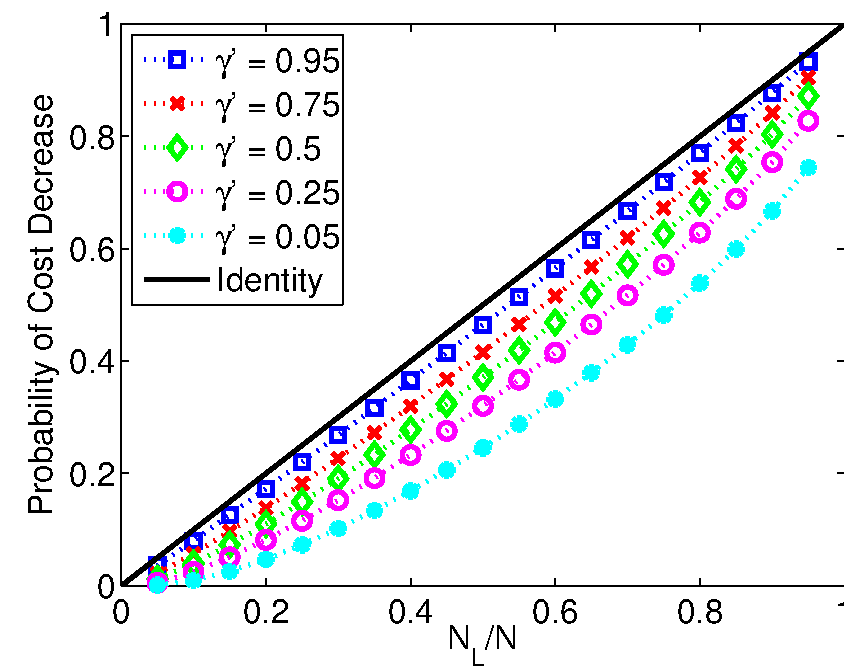
\includegraphics[width=.5\textwidth]{images/prob_dec_cost_v_nl_n_20}
	\caption{The probability that an additional sample decreases the optimal cost of the \plp\ as a function of the ratio $\frac{N_L}{N}$ for total sample size $N = 20$.}
	\label{fig:prob_cost_decrease_nd_n}
\end{figure}

\begin{figure}
	\centering
	\begin{subfigure}{.5\textwidth}
	   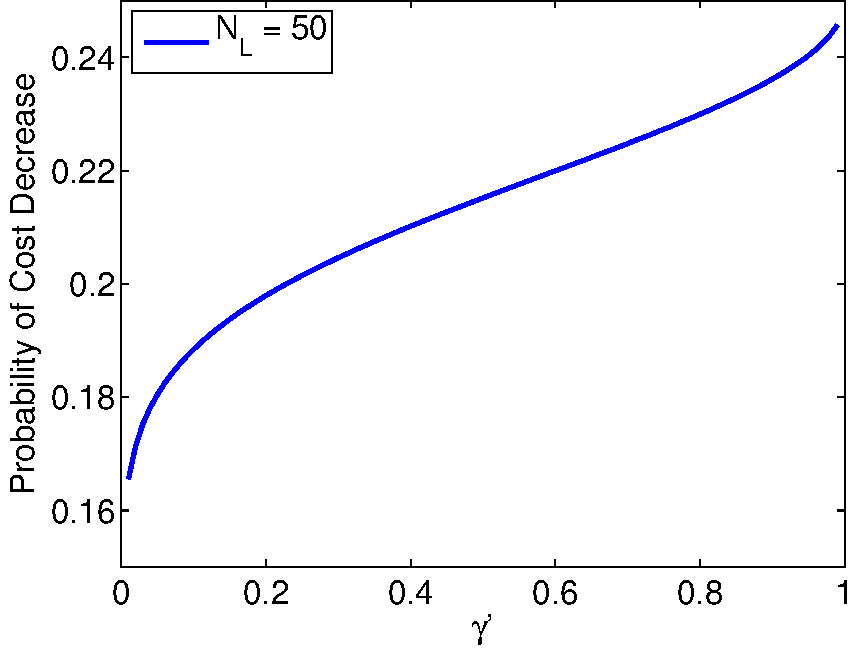
\includegraphics[width=\textwidth]{images/prob_dec_cost_v_gammaprime_no_context}
	   \caption{
			$N_L=50$ $\left(\frac{N_L}{N} = 0.25\right)$
		}
	   \label{fig:prob_cost_decrease_gp}
	\end{subfigure}%
	\begin{subfigure}{.5\textwidth}
	   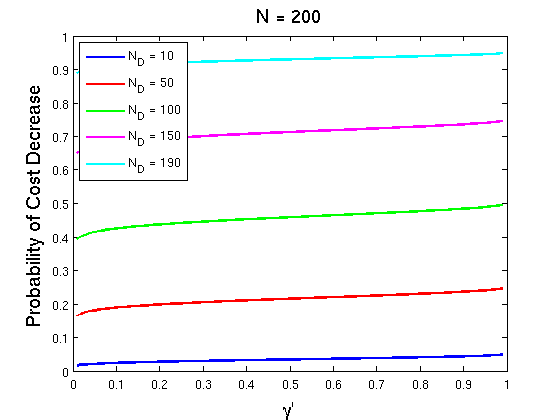
\includegraphics[width=\textwidth]{images/prob_dec_cost_v_gammaprime_no_context_multiple}
	   \caption{
			$N_L=10,50,100,150$ and $190$
		}
	   \label{fig:prob_cost_decrease_gp_multiple}
	\end{subfigure}%
	\caption{The probability that an additional sample decreases the optimal cost of the \plp\ as a function of $\gamma'$ for total sample size $N = 200$, (a) for a single value of $N_L = 50$ and (b) for multiple values of $N_L$.}
\end{figure}

Notice, however, that the three parameters discussed, $\gamma'$, $N$, and $N_L$ do not play the same role in the \plp.
The first two of these parameters are also parameters of the \plp\ problem (\ref{eq:plp_two_stage}).
The third, $N_L$, is computed from the optimal solution of (\ref{eq:plp_two_stage}) via (\ref{eq:p_worst}) and (\ref{eq:cost_decrease_cond}).
As such, $N_L$ should be viewed as changing with $\gamma'$.
In general, $N_L$ will decrease as $\gamma'$ increases. To see this, recall that values of  $\gamma'$ close to $1$ consider increasingly limited set of distributions, the ones closest to the maximum likelihood distribution $p_\omega = \frac{N_\omega}{N}$, $\forall \omega$. So, the condition given in (\ref{eq:cost_decrease_cond}) is satisfied for a smaller number of scenarios. As $N_L$ changes, the estimated bound on the probability of cost decrease will have one or more jump discontinuities, moving from one line to another line below it in Figure \ref{fig:prob_cost_decrease_gp_multiple}, as seen in Figure \ref{fig:water_prob_decrease}.
This behavior is studied in Section \ref{sec:comp_results}.

%%%%%%%%%%%%%%%%%%%%%%%%%%%%%%%%%%%%%%%%%%%%%%%%%%%%%%%%%%%%%%%%%%%%%%%%%%%%%%%%
\section{Asymptotic Analysis of \plp}
\label{sec:epiconvergence}

We now wish to show that the optimal value and solution of \plp\ converges to the optimal value and solution of the corresponding SLP-2 with the (unknown) true distribution $\ptrue$.
We begin by showing that the worst-case distribution converges weakly to the true distribution as $N \rightarrow \infty$.

Let the probability space $(\Xi,{\cal F},\P^\infty)$ be the space associated with taking infinitely many samples from the distribution $\ptrue$.
Let $\Xi' \subset \Xi$ be a measure 1 set such that $\hat{p}^N_\omega(\xi) \rightarrow \ptrue_\omega$ for all $\omega = 1, \dots, n$.

\begin{proposition} \label{prop:weak_conv}
	Let $p \neq \ptrue$.  For all $\epsilon > 0$ and $\xi \in \Xi'$ there exists $N'$ such that $\forall N \geq N'$ $D_{KL}(\hat{p}^N,p) \leq \frac{1}{N} \log\left(\frac{1}{\gamma'}\right) \Rightarrow \max_\omega |p_\omega - \ptrue_\omega| \leq \epsilon$.
\end{proposition}

\begin{proof}
	Without loss of generality, we assume that $\ptrue_\omega > 0$ for all $\omega$.
	This is valid because $\ptrue_\omega = 0 \Rightarrow \hat{p}^N_\omega = 0$, which implies $p_\omega = 0$ in the worst case distribution by (\ref{eq:p_worst}).
	For simplicity, we additionally assume $\epsilon$ is chosen so that $\ptrue_\omega > \frac{\epsilon}{2}$ for all $\omega$.
	
	First, we note that $\max_\omega |p_\omega - \ptrue_\omega| \leq \max_\omega |p_\omega - \hat{p}^N_\omega| + \max_\omega |\hat{p}^N_\omega - \ptrue_\omega|$.
	Let $N''$ be such that $\max_\omega |\hat{p}^N_\omega - \ptrue_\omega| \leq \frac{\epsilon}{2}$ for all $N \geq N''$.
	
	Next, we use the alternate form of the KL divergence
	\[
		D_{KL}(\hat{p}^N,p) = \sum_{\omega=1}^n \hat{p}^N_\omega \left( - \log \frac{p_\omega}{\hat{p}^N_\omega} + \frac{p_\omega}{\hat{p}^N_\omega} - 1 \right),
	\]
	and use the fact that each term in parentheses $\phi(t) = -\log t + t - 1$ is convex, non-negative for $t \geq 0$, and $\phi(1) = 0$.
	
	To complete the proof, we will show that one can choose $N' \geq N''$ such that $\forall N \geq N'$, $\max_\omega |p_\omega - \hat{p}^N_\omega| > \frac{\epsilon}{2} \Rightarrow D_{KL}(\hat{p}^N,p) > \frac{1}{N} \log\left(\frac{1}{\gamma'}\right)$.
	First, bound the KL divergence by
	\begin{align*}
		D_{KL}(\hat{p}^N,p) & = \sum_{\omega=1}^n \hat{p}^N_\omega \phi\left( \frac{p_\omega}{\hat{p}^N_\omega} \right) \\
		& \geq \min_\omega \{\hat{p}^N_\omega\} \cdot \max_\omega \left\{ \phi \left( \frac{p_\omega}{\hat{p}^N_\omega} \right) \right\} \\
		& \geq \min_\omega \{\hat{p}^N_\omega\} \cdot \min\left\{ \phi\left(1+\frac{\epsilon}{2}\right), \phi\left(1-\frac{\epsilon}{2}\right) \right\} \\
		& \geq \min_\omega \left\{ \ptrue_\omega - \frac{\epsilon}{2} \right\} \cdot \min\left\{ \phi\left(1+\frac{\epsilon}{2}\right), \phi\left(1-\frac{\epsilon}{2}\right) \right\},
	\end{align*}
	where the second inequality is true because $\phi \left( \frac{p_\omega}{\hat{p}^N_\omega} \right) \geq \min\left\{ \phi\left( \frac{\hat{p}^N_\omega+\tfrac{\epsilon}{2}}{\hat{p}^N_\omega} \right), \phi\left( \frac{\hat{p}^N_\omega-\tfrac{\epsilon}{2}}{\hat{p}^N_\omega} \right) \right\}$ for at least one $\omega$, and applying the inequalities $\frac{a+\eta}{a} \geq 1 + \eta$ and $\frac{a-\eta}{a} \leq 1-\eta$.
	Then choose $N'$ to satisfy $\min_\omega \left\{ \ptrue_\omega - \frac{\epsilon}{2} \right\} \cdot \min\left\{ \phi\left(1+\frac{\epsilon}{2}\right), \phi\left(1-\frac{\epsilon}{2}\right) \right\} \geq \frac{1}{N'} \log\left(\frac{1}{\gamma'}\right)$.
\end{proof}

Proposition \ref{prop:weak_conv} shows that the worst-case distributions of (\ref{eq:plp_primal}) converge weakly to $\ptrue$.
In the next theorem, we establish the proof that the optimal value and solution of \plp\ converges to that of the SLP-2 with distribution $\ptrue$ by establishing the epiconvergence of \plp\ to SLP-2.
\begin{theorem}
	\plp\ (\ref{eq:plp_two_stage}) epiconverges to SLP-2 (\ref{eq:slp_first_stage}) with distribution $p = \ptrue$.
\end{theorem}

\begin{proof}
	To establish the epiconvergence, we need only to apply the result of Proposition \ref{prop:weak_conv} to Theorem 3.7 of \cite{dupacova1988asymptotic}, which establishes the epiconvergence of (\ref{eq:plp_primal}) under the evident conditions that the objective function (under the worst-case distribution) is continuous with respect to $\omega$ and lower semicontinuous and locally lower Lipschitz with respect to $x$.
\end{proof}

%%%%%%%%%%%%%%%%%%%%%%%%%%%%%%%%%%%%%%%%%%%%%%%%%%%%%%%%%%%%%%%%%%%%%%%%%%%%%%%%
\section{Decomposition-Based Solution Method} \label{sec:soln_algorithm}

As the model gets larger, as in our water application presented in Section~\ref{sec:comp_results}, a direct solution of \plp\ becomes computationally expensive. 
Decomposition-based methods could significantly reduce the solution time and allow for larger problems to be solved efficiently. In this section, we propose a Bender's decomposition-based method for solving \plp.
Our algorithm uses the \plp\ second-stage problems $h_\omega(\x,\lambda,\mu)$ (\ref{eq:plp_second_stage}) to form the cuts, ensuring a linear master problem.
The algorithm removes constraint (\ref{eq:plp_feas_constraint}) from the second-stage problem (\ref{eq:plp_second_stage}) and exchanges it with a series of feasibility constraints (or cuts) in the first-stage problem.
Making this change ensures that the second-stage problems are solved using the formulation of $h^\dagger_\omega(\x)$ for SLP-2 given in  (\ref{eq:slp_second_stage}), and is more efficient.
The master problem is given by
\begin{align}
	\min_{\x,\lambda,\mu} \ & \c\x + \mu + \bar{N}\lambda + \theta \label{eq:master_problem}\\
	\st \ & A\x = \b \nonumber \\
	& \theta \geq T_j (\x,\lambda,\mu)^T + t_j, \ j \in J \nonumber \\
	& \mu \geq M_k \x + m_k, \ k \in K \nonumber \\
	& \x,\lambda \geq 0, \nonumber
\end{align}
where $T_j (\x,\lambda,\mu)^T + t_j$ are the objective cuts, $M_k \x + m_k$ are the feasibility cuts on constraint (\ref{eq:plp_feas_constraint}), and $J$ and $K$ are the sets of objective and feasibility cuts, respectively.
The proposed algorithm follows.
For details on its derivation, see \cite{love2013likelihood}.

\subsection{Objective Cuts}

Let $(\xh,\lh,\mh)$ be the candidate solution from the master problem (\ref{eq:master_problem}).
An objective cut can be computed by solving the SLP-2 subproblems $h^\dagger_\omega(\xh)$ along with optimal dual solutions $\pi^{*,\omega}$ to each second-stage problem, and using these to compute the partial (sub)derivatives of the \plp\ subproblems as
\begin{align*}
	\dfrac{\partial h_\omega}{\partial \x}(\xh,\lh,\mh) & = \left(\dfrac{N\lh}{\mh - h^\dagger_\omega(\xh)}\right) \pi^{*,\omega} B^\omega \\
	\dfrac{\partial h_\omega}{\partial \lambda}(\xh,\lh,\mh) & = N + N\log\lh - N \log(\mh - h^\dagger_\omega(\xh)) \\
	\dfrac{\partial h_\omega}{\partial \mu}(\xh,\lh,\mh) & = \dfrac{-N\lh}{\mh - h^\dagger_\omega(\xh)}
\end{align*}
Recall that $h^\dagger_\omega(\x) = \min_{y^\omega \geq 0} \{\q^\omega y^\omega | D^\omega y^\omega = \d^\omega + B^\omega \x\}$.
The cuts are then given by
\begin{align*}
	T_j^\omega & = 
	\left( \begin{array}{ccc}
		\left(\frac{N\lh}{\mh - h^\dagger_\omega(\xh)}\right) \pi^{*,\omega} B^\omega, 
			 & N + N\log\lh - N\log(\mh - h^\dagger_\omega(\xh)), 
			 & -\frac{N\lh}{\mh - h^\dagger_\omega(\xh)}
	\end{array} \right) \\
	t_j^\omega & = \frac{N \lh h^\dagger_\omega(\xh) - N \lh \pi^{*,\omega}B\xh}{\mh - h^\dagger_\omega(\xh)}.
\end{align*}

For the single-cut master problem proposed, $T_j = \sum_\omega \frac{N_\omega}{N} T_j^\omega$ and $t_j = \sum_\omega \frac{N_\omega}{N} t_j^\omega$.

\subsection{Feasibility Cuts}
After the subproblems $h^\dagger_\omega(\xh)$ are solved, it may be the case that $\mh - h^\dagger_\omega(\xh) < 0$ for some $\omega$, rendering $\mh$ infeasible.
This is corrected using the feasibility problem
\begin{align*}
	U_\omega(\x,\mu) = \min_{y_\omega,z \geq 0} \ & z \\
	\st \ & z + \mu - \q^\omega y^\omega \geq 0 \\
	& D^\omega y^\omega = \d^\omega + B^\omega \x,
\end{align*}
which is solved by $z^* = h^\dagger_\omega(\x) - \mu$.
The subdifferentials can be easily found as $\frac{\partial z^*}{\partial \x} = \pi^{*,\omega} B^\omega$ and $\frac{\partial z^*}{\partial \mu} = -1$.
Then for infeasible candidate solution $(\xh,\lh,\mh)$ we get the inequality
\begin{align*}
	U_\omega(\x,\mu) \geq \pi^{*,\omega}B^\omega(\x-\xh) - (\mu -\mh) + h^\dagger_\omega(\xh) - \mh,
\end{align*}
and setting $U_\omega(\x,\mu) = 0$ to find a feasible solution gives the feasibility cut
\[
	\mu \geq \pi^{*,\omega}B^\omega \x + (h^\dagger_\omega(\xh) - \pi^{*,\omega}B^\omega\xh).
\]

Once the feasibility cut is generated, we may need to find a feasible (and reasonable) value of $\mu$ to generate an objective cut, or to initialize the next iteration of the master problem.
This can be done quickly by minimizing the objective function of (\ref{eq:plp_det_equiv}) with respect to $\mu$ while keeping $\xh$ and $\lh$ constant, which is equivalent to minimizing $\mu - \sum_\omega N_\omega \lh \log(\mu - h^\dagger_\omega(\xh))$.
We do this by solving the equation $\sum_\omega \frac{N_\omega \lh}{\mu - h^\dagger_\omega(\xh)} = 1$ with Newton's method.

\subsection{Decomposition Algorithm}

We solve the \plp\ with the following decomposition algorithm with tolerance level $\texttt{TOL}$

% \begin{figure}
	\begin{algorithmic}
		\State Initialize $z_l = -\infty, z_u = \infty$
		\State Solve first stage (\ref{eq:master_problem}) with $\theta = 0$  to generate $\x$
		\State Solve all second stage scenarios $h^\dagger_\omega(\x)$ (\ref{eq:slp_second_stage})
		\State Initialize $\lambda \gets 1$, $\mu$ that minimizes $\mu - \sum_\omega N_\omega \lh \log(\mu - h^\dagger_\omega(\xh))$
		\State Generate initial objective cut
		\While{$z_u - z_l \geq \texttt{TOL}\min\{|z_u|,|z_l|\}$}
			\State Solve master problem (\ref{eq:master_problem}), get $\x$,$\lambda$,$\mu$,$\theta_M$
			\State Solve sub-problems $h^\dagger_\omega(\x)$ (\ref{eq:slp_second_stage})
			\State $\theta_{\text{true}} \gets \sum_{\omega=1}^n \frac{N_\omega}{N} h_\omega(\x,\lambda,\mu)$
			\If{$\mu < \max_\omega h^\dagger_\omega(\x)$}
				\State Generate feasibility cut
				\State Find $\mu$ that minimizes $\mu - \sum_\omega N_\omega \lh \log(\mu - h^\dagger_\omega(\xh))$
			\Else
				\State $z_l \gets$ master optimal cost $\c\x + \mu + \bar{N}\lambda + \theta_{\text{true}}$
			\EndIf
			\State Generate objective cut
			\If{$\c\x + \mu + \bar{N}\lambda + \theta_{\text{true}} < z_u$}
				\State $z_u \gets \c\x + \mu + \bar{N}\lambda + \theta_{\text{true}}$
				\State $\x_\text{best} \gets \x, \lambda_\text{best} \gets \lambda, \mu_\text{best} \gets \mu$
				\State $p_\omega \gets \frac{\lambda_\text{best} N_\omega}{\mu_\text{best} - h^\dagger_\omega(\x_\text{best})}$ for $i = 1, \dots, n$
			\EndIf
		\EndWhile
	\end{algorithmic}
% 	\caption{Proposed Bender's Decomposition algorithm for solving \plp}
% 	\label{fig:algorithm}
% \end{figure}

\subsection{Computational Enhancements}

In order to enhance the performance of the above decomposition-based algorithm, we made some adjustments.
First, we included an $L_\infty$-norm trust region which is scaled up (by a factor of $3$) or down (by a factor of $\tfrac{1}{4}$) when the trust region inhibits finding the optimal solution or when the polyhedral lower approximation is far from the second-stage expected cost, respectively.
The trust region is an implementation of Algorithm 4.1 in \cite{nocedal1999numerical}.

Because we are also interested in the worst-case LRO probabilities given in the primal variables and not computed directly, we include a second tolerance as a stopping condition, ensuring that $\left| 1 - \sum_{i=1}^n p_\omega \right| < \texttt{TOL2}$ when the algorithm is completed.
This must be satisfied in addition to the original condition $z_u - z_l < \texttt{TOL}\min\{|z_u|,|z_l|\}$.

%%%%%%%%%%%%%%%%%%%%%%%%%%%%%%%%%%%%%%%%%%%%%%%%%%%%%%%%%%%%%%%%%%%%%%%%%%%%%%%%
\section{Application and Computational Results} \label{sec:comp_results}

\subsection{Generalized Network Water Model} 
\label{ssec:network_model}

We applied \plp\ to a multi-period generalized network flow model of Colorado River water allocation in Tucson, defined by a set of nodes and directed arcs $(N,\: A)$.
The nodes represent available water supply from the Colorado River, water treatment plants, reservoirs, and water demand sites.
The arcs represent the conveyance system (pipes, etc.) that carry water between the nodes. 
Water can be stored in between time periods in reservoirs to meet future demands. 
The model aims to find the minimal cost water flows considering energy, treatment, storage, and transportation costs over the planning period. 
Generalized network water allocation models have been used to find water allocations and delivery reliabilities and to assess values of different water use operations; see, e.g., \cite{draper_etal_03}. 

Water flows on arc $(i,j) \in A$ during time period $t = 1, \dots, P$ are represented by decisions $x_{ijt}$.
Each arc $(i,j) \in A$ and time period $t$ has a unit cost $c_{ijt}^x$, loss coefficient $0 \leq a_{ijt} \leq 1$ to account for evaporation, leakage from the pipes, etc., and bounds on the flow $l_{ijt}^x \leq x_{ijt} \leq u_{ijt}^x$.
Each node $j \in N$ has a supply/demand for time period $t$, $b_{jt}$.
Nodes representing reservoirs are able to store water between time periods.
Stored water available at node $j$ at the beginning of time period $t$ is $s_{jt}$, with associated cost $c_{jt}^s$ and bounds $l_{jt}^s \leq s_{jt} \leq u_{jt}^s$.
Finally, water released into the environment from node $j$ in period $t$ is given by $r_{jt}$, with bounds $l_{jt}^r \leq r_{jt} \leq u_{jt}^r$.
The deterministic model is a multi-period generalized network flow model of the form
\begin{align*}
	\min_{x,s,r} \ & \sum_{(i,j) \in A} \sum_{t=1}^P c_{ijt}^x x_{ijt} + \sum_{j \in N} \sum_{t=1}^P c_{jt}^s s_{jt}\\
	\st \ & \sum_{i \in N} x_{jit} + s_{j,t+1} + r_{jt} = \sum_{i \in N} a_{ijt} x_{ijt} + s_{jt} + b_{jt}, \ \ \forall j,t \\
	& l_{ijt}^x \leq x_{ijt} \leq u_{ijt}^x,\ \ \ \forall i,j,t \\
	& l_{jt}^s \leq s_{jt} \leq u_{sjt}^s, \ \ \ \forall j,t \\
	& l_{jt}^r \leq r_{jt} \leq u_{sjt}^r, \ \ \ \forall j,t.
\end{align*}

The model is converted to a two-stage stochastic model with $P_1$ periods in the first stage and $P-P_1$ stages in the second stage.
We assume that the supplies and demands are uncertain, as well as the bounds on the decision variables.
\begin{align}
	\min_{(x,s,r) \in L^1} \ & \sum_{(i,j) \in A} \sum_{t=1}^{P_1} c_{ijt}^x x_{ijt} + \sum_{j \in N} \sum_{t=1}^{P_1} c_{jt}^s s_{jt} + \sum_{\omega=1}^n p_\omega h^\dagger_\omega(s) \label{eq:gen_network_two_stage} \\
	\st \ & \sum_{i \in N} x_{jit} + s_{j,t+1} + r_{jt} = \sum_{i \in N} a_{ijt} x_{ijt} + s_{jt} + b_{jt},\ \ \ \ \forall j, 1 \leq t \leq P_1, \notag
\end{align}
where the second stage problems
\begin{align}
	h^\dagger_\omega(s) = \min_{(x,s,r) \in L^2_\omega} \ & \sum_{(i,j) \in A} \sum_{t=P_1+1}^{P} c_{ijt}^x x_{ijt} + \sum_{j \in N} \sum_{t=P_1+1}^{P} c_{jt}^s s_{jt} \label{eq:gen_network_second_stage} \\
	\st \ & \sum_{i \in N} x_{jit} + s_{j,t+1} + r_{jt} = \sum_{i \in N} a_{ijt} x_{ijt} + s_{jt} + b_{jt}^\omega, \ \ \ \ \forall j, P_1+1 \leq t \leq P, \notag
\end{align}
and $L^1$ and $L^2_\omega$ represent the feasible regions defined by the lower and upper variable bounds.

% In the rest of the paper, we simplify the notation for the first-stage (\ref{eq:gen_network_two_stage}) and second-stage (\ref{eq:gen_network_second_stage}) problems as follows.
% In the first stage, decision variables $\{x_{ijt}\}$, $\{s_{jt}\}$ and $\{r_{jt}\}$ become the vector $\x$, costs $\{c_{ijt}^x\}$ and $\{c_{jt}^s\}$ are written as the row vector $\c$, the supply/demand parameters $b_{jt}$ become the vector $\b$ and the constraint matrix is written as $A$.
% In the second stage, we denote the decisions as $\y^\omega$, the costs as $\q^\omega$, the supply/demands as $\d^\omega$, and the constraint matrices multiplying $\y^\omega$ and $\x$ as $D^\omega$ and $B^\omega$, respectively.

% Using the generalized network model (\ref{eq:gen_network_two_stage}) of Colorado River water allocation in the southeastern portion of Tucson, we created a likelihood robust water allocation problem of the form \plp.
% The southeastern portion of Tucson is a newly developing area and is expected to grow considerably. 
% The \plp\ water allocation model would help authorities with future water plans in this area while being robust to uncertainties in water supplies and demands.

The model has a total of $P = 41$ time periods, representing years 2010--2050. 
%, with projections coming from studies WISP \cite{??} and TAZ \cite{??}.
% We use $P_1 = 10$ time periods for the first stage, and four second-stage scenarios are constructed from high (WISP) and low (TAZ) population estimates along with high and low estimates for the amount of water available for use.
For each time period, the network has 62 nodes representing demand for potable and nonpotable (reclaimed) water, pumps, water treatment plants, and the available water supply from the Colorado River.
The network in each time period has 102 arcs, representing the pipe network carrying the water between the nodes physically and connecting the network to the five reservoirs that connect the time stages in the model.
We use $P_1 = 10$ time periods for the first stage.
Uncertainty in the second stage takes the form of uncertain population (thus, demand for water) and supply of water.
There are a total of 4 scenarios considered in this test instance: (i) high population, high supply, (ii) high population, low supply, (iii) low population, high supply, and (iv) low population, low supply.
Each scenario is assumed to have five observations.
The high population scenarios are more costly as the system needs to meet demand or pay for unmet demand.
The low population scenarios, on the other hand, are not as costly. 
% The supply variability seems to have a nominal effect.
We applied the decomposition-based solution algorithm presented in Section \ref{sec:soln_algorithm} to solve this model.% and selected tolerances $\texttt{TOL} = 10^{-5}$ and $\texttt{TOL2} = 10^{-3}$ for our computational experiments.

\subsection{Computational Results}

Figure \ref{fig:worst_case} shows how the worst-case distribution changes with $\gamma'$.
When $\gamma'$ is close to $1$, we use the maximum likelihood distribution, which has equal $\tfrac{1}{4}$ probabilities on each of the four scenarios.
As $\gamma'$ is decreased, the ambiguity set increases, and the worst-case distribution used by \plp\ changes.
It gives higher than $\tfrac{1}{4}$ probability to the two high-population scenarios and lower than $\tfrac{1}{4}$ probability to the two low-population scenarios, making the solution more robust to costly scenarios.
Note that the scenarios fall into two similar pairs because the cost of each scenario depends strongly on the projected demand but only weakly on the projected supply of Colorado River water.
A closer look at the optimal solutions reveals that as $\gamma'$ is decreased, or as robustness is increased, the solution uses more and more reclaimed water (treated wastewater that is reused for nonpotable purposes such as irrigation) in an effort to meet demands in a least-costly way.

\begin{figure}
	\centering
	\begin{subfigure}{.5\textwidth}
		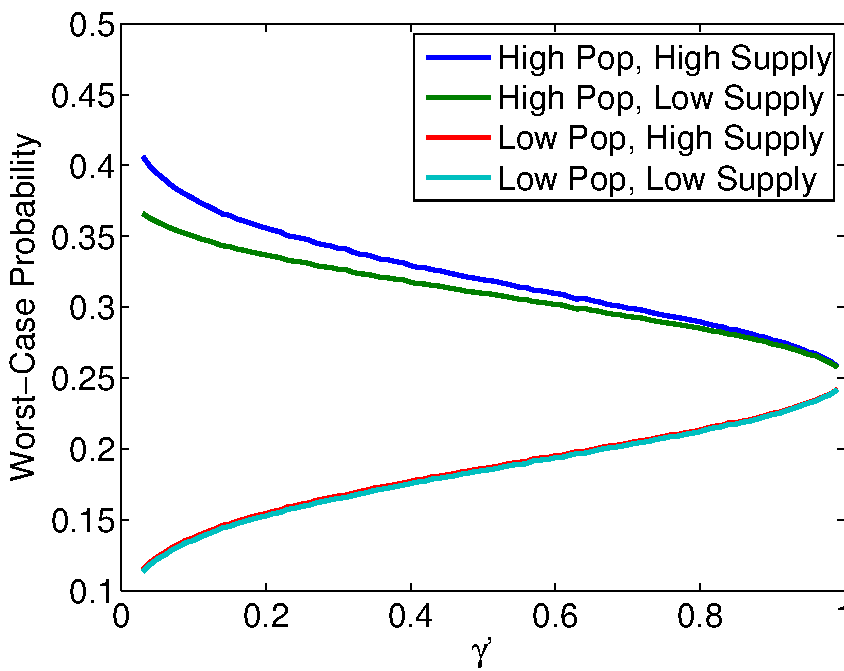
\includegraphics[width=\textwidth]{images/worst_case_probability}
		\caption{Worst case distributions}
		\label{fig:worst_case}
	\end{subfigure}%
	\begin{subfigure}{.5\textwidth}
		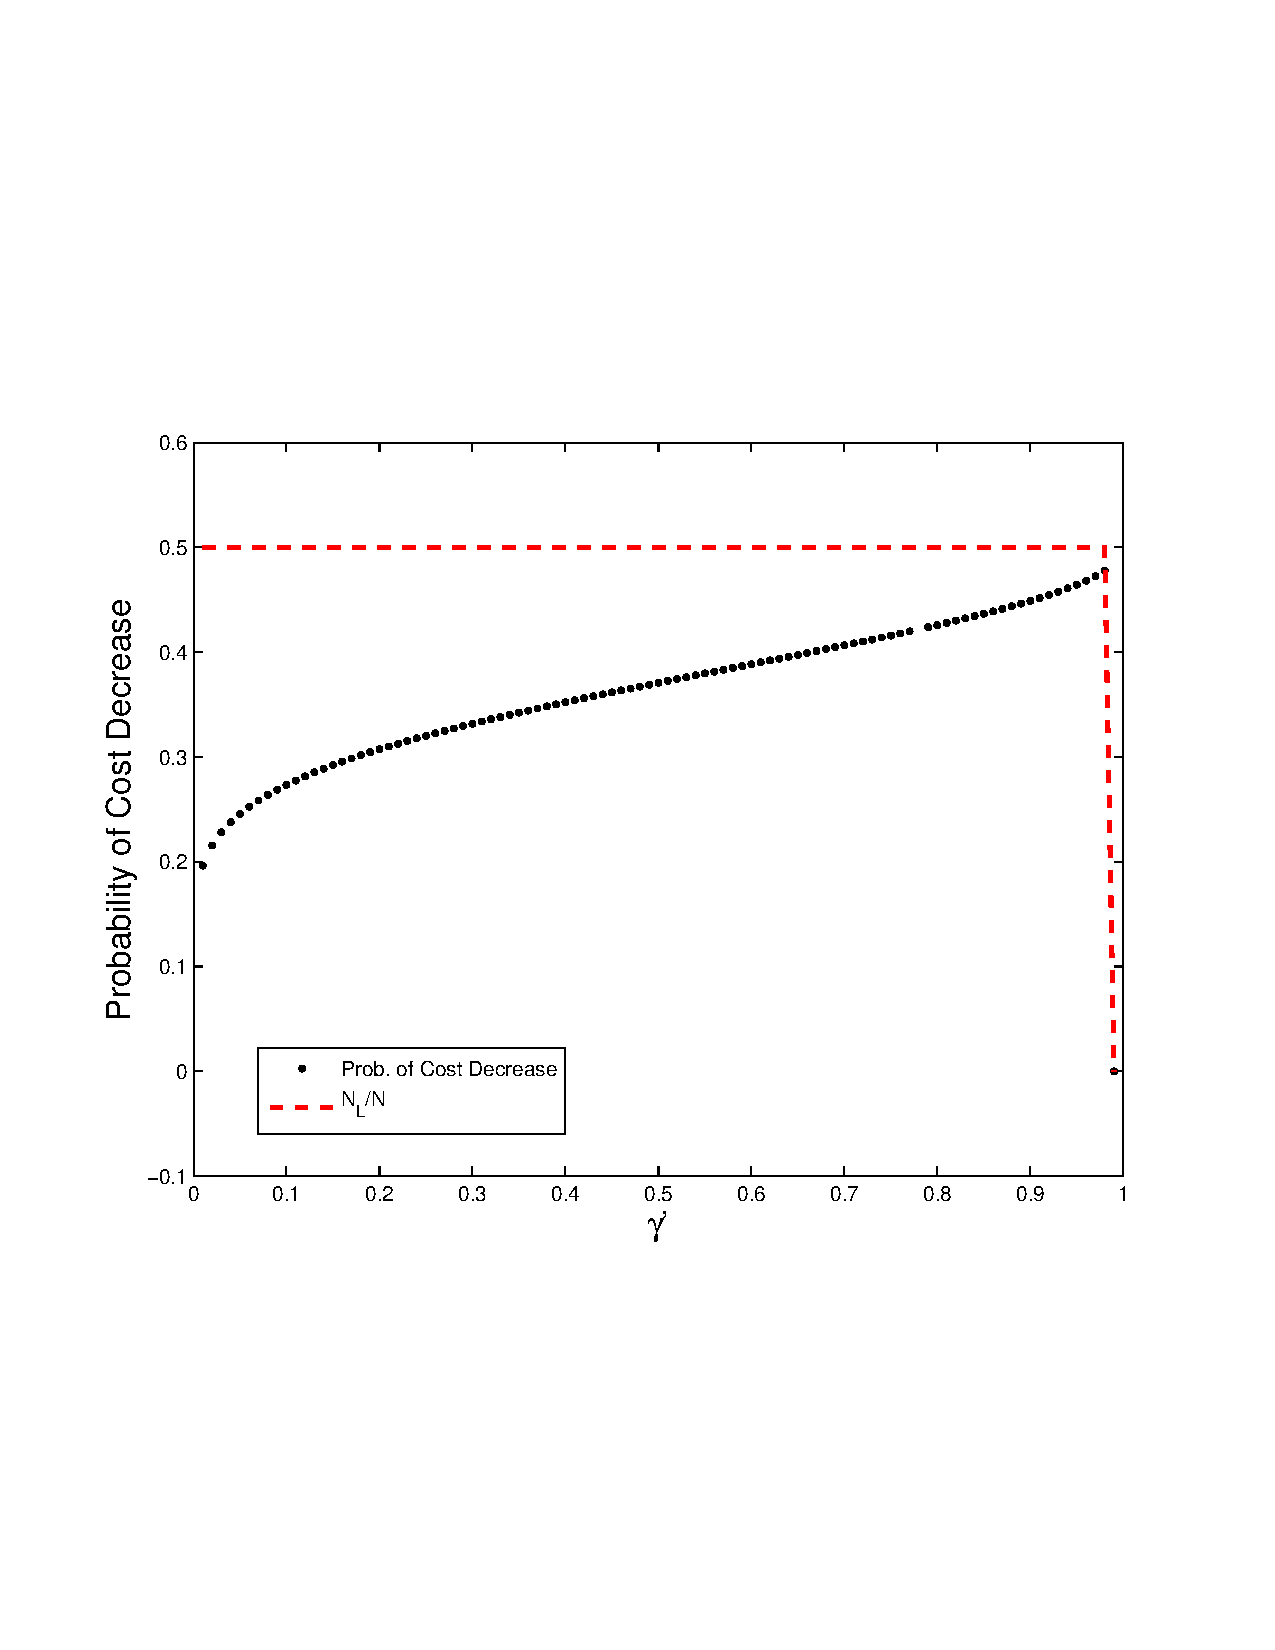
\includegraphics[width=\textwidth]{images/water_prob_decrease}
		\caption{Probability of cost decrease}
		\label{fig:water_prob_decrease}
	\end{subfigure}
	\caption{%
		(a) Worst-case distribution for the likelihood robust water allocation problem.
		(b) Probability that an additional sample causes a decrease in worst-case expected cost for the likelihood robust water allocation problem.
		The red line shows the upper bound probability $\tfrac{N_L}{N}$.
	}
\end{figure}

%\subsection{Value of Data}

The results of the water model were then analyzed with the value of data techniques from Section \ref{sec:value}.
Figure \ref{fig:water_prob_decrease} shows the estimated probability that an additional sample will remove the worst-case distribution from the likelihood region, resulting in a lower-cost solution. %, analogous the results of Figure \ref{fig:prob_cost_decrease_gp}.
The dashed line in Figure \ref{fig:water_prob_decrease} depicts the computed values of $\frac{N_L}{N}$, which provide an upper bound on the estimated probabilities. 
Because the low-population scenarios have lower costs, an additional sample of either low-population scenario will result in a lower expected cost.
This is what we see through most of the computed values of $\gamma'$, with $\frac{N_L}{N} = 0.5$, indicating that the sufficient condition (\ref{eq:cost_decrease_cond}) was satisfied for both low-population scenarios.
For extremely large values of $\gamma'$---above $0.97$---we see the ratio $\frac{N_L}{N}$ quickly drops to zero.
This occurs because (\ref{eq:cost_decrease_cond}) only compares scenario probabilities in the empirical ($N_\omega / N$) and worst-case ($p_\omega$) distributions and does not use the computed cost of the scenarios.
As $\gamma'$ increases and the ambiguity set shrinks, the worst-case probabilities become so close the empirical probabilities that (\ref{eq:cost_decrease_cond}) can no longer be satisfied, resulting in $\frac{N_L}{N}$ decreasing to zero.
% 
% \begin{figure}
% 	\centering
% 	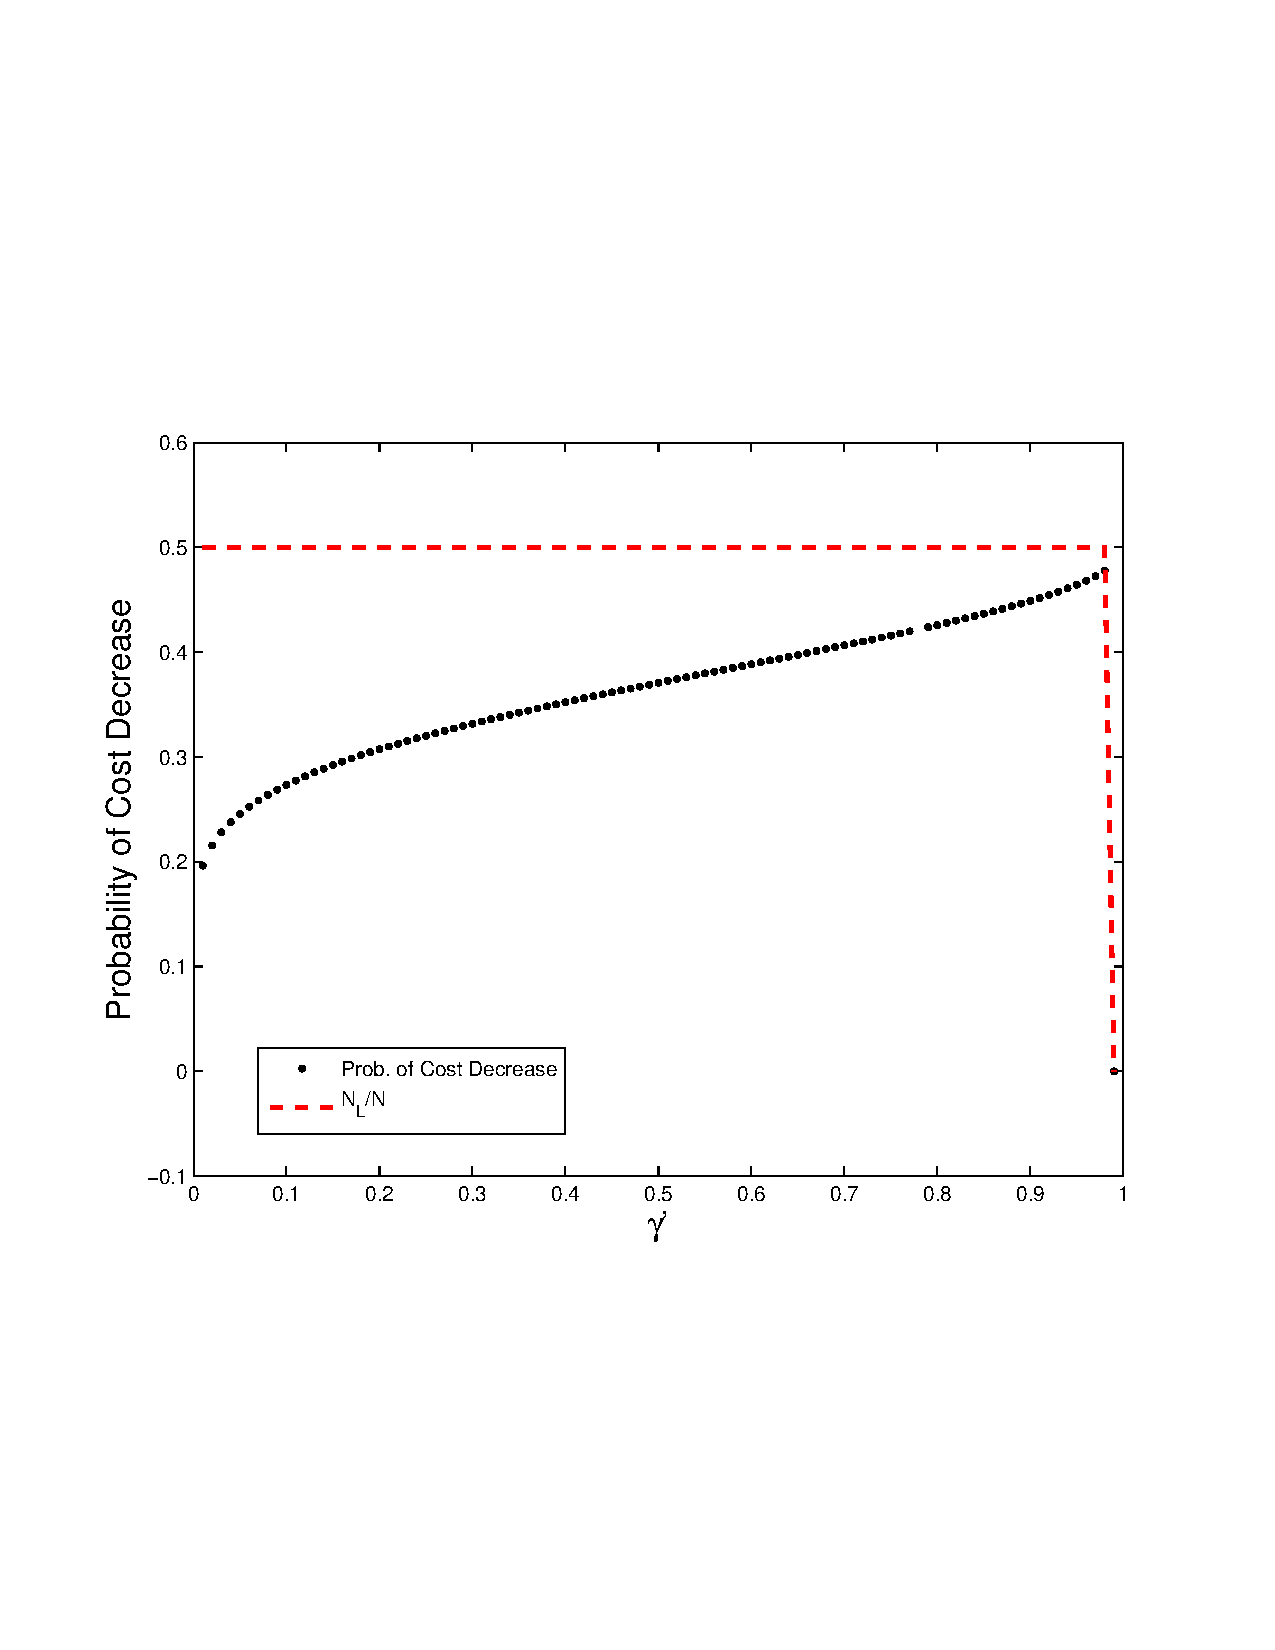
\includegraphics[width=.5\textwidth]{images/water_prob_decrease}
% 	\caption{Probability that an additional sample causes a decrease in worst-case expected cost for the likelihood robust water allocation problem.  The red line shows the upper bound probability $\tfrac{N_L}{N}$.}
% 	\label{fig:water_prob_decrease}
% \end{figure}

%%%%%%%%%%%%%%%%%%%%%%%%%%%%%%%%%%%%%%%%%%%%%%%%%%%%%%%%%%%%%%%%%%%%%%%%%%%%%%%%
\section{Conclusion and Future Work}
\label{sec:concl}

In this paper, we proposed an extension of the Likelihood Robust Optimization (LRO) method of Wang et al.\ \cite{wang2010likelihood} to general two-stage stochastic programs with recourse, creating a two-stage likelihood robust program with recourse, denoted \plp.
The LRO models use the empirical likelihood function to define an ambiguity set of probability distributions using observed data and optimize the worst-case expected cost with respect to this likelihood ambiguity set.
We provided a computationally simple method to estimate the probability that an additional sample will produce a likelihood ambiguity set that does not contain the current worst-case distribution and will result in a lower-cost solution. 
We have also provided a Bender's decomposition-based solution algorithm for the \plp\ and applied this method to planning future water distribution in Tucson, Arizona.

Our future work includes the following. We plan to augment the existing model first with a richer set of second-stage scenarios.
In addition to more varied estimates for future population, we will integrate climate change predictions into the model to generate scenarios for future water supply from the Colorado River. 
This model is intended to include a facility location problem to determine the best places for an additional waste water treatment plants to increase the use of reclaimed water in the most cost-efficient manner. On the methodological side, we plan to generalize our results to the more general $\phi$-divergence case of \cite{bental2011robust}.

\section*{Acknowledgements}
Support provided by a Water Sustainability Program Fellowship through the Technology and Research Initiative Fund at the University of Arizona.
This work has also been partially supported by the National Science Foundation through grant CMMI-1151226.

An earlier version of this paper appeared in the Proceedings of the 2013 Industrial and Systems Engineering Research Conference \cite{love2013likelihood}.

\bibliography{love_lro}



\section*{Author Biographies}

\noindent {\bf DAVID LOVE} is a graduate student in the Graduate Interdisciplinary Program in Applied Mathematics at the University of Arizona.
His research interests include distributionally robust stochastic programming and water resources management.
His email address is \url{dlove@math.arizona.edu} and his web page is \url{http://math.arizona.edu/~dlove}.

\bigskip

\noindent {\bf G\"{U}ZIN BAYRAKSAN} is an Associate Professor of Integrated Systems Engineering at the Ohio State University.
Her research interests include Monte Carlo sampling methods for stochastic programming and applications to water resources.
Her email address is \url{bayraksan.1@osu.edu} and her web page is \url{http://www-iwse.eng.ohio-state.edu/biosketch_GBayraksan.cfm}

\end{document}
